\documentclass[12pt]{article}

\usepackage{amsthm}
\usepackage{amsmath}
\usepackage{amsfonts}
\usepackage{mathrsfs}
\usepackage{array}
\usepackage{amssymb}
\usepackage{units}
\usepackage{graphicx}
\usepackage{tikz-cd}
\usepackage{nicefrac}
\usepackage{hyperref}
\usepackage{bbm}
\usepackage{color}
\usepackage{tensor}
\usepackage{tipa}
\usepackage{bussproofs}
\usepackage{ stmaryrd }
\usepackage{ textcomp }
\usepackage{leftidx}
\usepackage{afterpage}
\usepackage{varwidth}
\usepackage{tasks}
\usepackage{ cmll }

\newcommand\blankpage{
    \null
    \thispagestyle{empty}
    \addtocounter{page}{-1}
    \newpage
    }

\graphicspath{ {images/} }

\theoremstyle{plain}
\newtheorem{thm}{Theorem}[subsection] % reset theorem numbering for each chapter
\newtheorem{proposition}[thm]{Proposition}
\newtheorem{lemma}[thm]{Lemma}
\newtheorem{fact}[thm]{Fact}
\newtheorem{cor}[thm]{Corollary}

\theoremstyle{definition}
\newtheorem{defn}[thm]{Definition} % definition numbers are dependent on theorem numbers
\newtheorem{exmp}[thm]{Example} % same for example numbers
\newtheorem{notation}[thm]{Notation}
\newtheorem{remark}[thm]{Remark}
\newtheorem{condition}[thm]{Condition}
\newtheorem{question}[thm]{Question}
\newtheorem{construction}[thm]{Construction}
\newtheorem{exercise}[thm]{Exercise}
\newtheorem{example}[thm]{Example}
\newtheorem{aside}[thm]{Aside}

\def\doubleunderline#1{\underline{\underline{#1}}}
\newcommand{\bb}[1]{\mathbb{#1}}
\newcommand{\scr}[1]{\mathscr{#1}}
\newcommand{\call}[1]{\mathcal{#1}}
\newcommand{\psheaf}{\text{\underline{Set}}^{\scr{C}^{\text{op}}}}
\newcommand{\und}[1]{\underline{\hspace{#1 cm}}}
\newcommand{\adj}[1]{\text{\textopencorner}{#1}\text{\textcorner}}
\newcommand{\comment}[1]{}
\newcommand{\lto}{\longrightarrow}
\newcommand{\rone}{(\operatorname{R}\bold{1})}
\newcommand{\lone}{(\operatorname{L}\bold{1})}
\newcommand{\rimp}{(\operatorname{R} \multimap)}
\newcommand{\limp}{(\operatorname{L} \multimap)}
\newcommand{\rtensor}{(\operatorname{R}\otimes)}
\newcommand{\ltensor}{(\operatorname{L}\otimes)}
\newcommand{\rtrue}{(\operatorname{R}\top)}
\newcommand{\rwith}{(\operatorname{R}\&)}
\newcommand{\lwithleft}{(\operatorname{L}\&)_{\operatorname{left}}}
\newcommand{\lwithright}{(\operatorname{L}\&)_{\operatorname{right}}}
\newcommand{\rplusleft}{(\operatorname{R}\oplus)_{\operatorname{left}}}
\newcommand{\rplusright}{(\operatorname{R}\oplus)_{\operatorname{right}}}
\newcommand{\lplus}{(\operatorname{L}\oplus)}
\newcommand{\prom}{(\operatorname{prom})}
\newcommand{\ctr}{(\operatorname{ctr})}
\newcommand{\der}{(\operatorname{der})}
\newcommand{\weak}{(\operatorname{weak})}
\newcommand{\exi}{(\operatorname{exists})}
\newcommand{\fa}{(\operatorname{for\text{ }all})}
\newcommand{\ex}{(\operatorname{ex})}
\newcommand{\cut}{(\operatorname{cut})}
\newcommand{\ax}{(\operatorname{ax})}
\newcommand{\negation}{\sim}
\newcommand{\true}{\top}
\newcommand{\false}{\bot}
\DeclareRobustCommand{\diamondtimes}{%
  \mathbin{\text{\rotatebox[origin=c]{45}{$\boxplus$}}}%
}
\newcommand{\tagarray}{\mbox{}\refstepcounter{equation}$(\theequation)$}
\newcommand{\startproof}[1]{
\AxiomC{#1}
\noLine
\UnaryInfC{$\vdots$}
}
\newenvironment{scprooftree}[1]%
  {\gdef\scalefactor{#1}\begin{center}\proofSkipAmount \leavevmode}%
  {\scalebox{\scalefactor}{\DisplayProof}\proofSkipAmount \end{center} }

\usepackage[margin=1cm]{geometry}


\title{Linear Logic}
\author{Will Troiani}
\date{February 2021}

\begin{document}
\maketitle
\tableofcontents
\section{Multiplicatives}
\begin{defn}\label{def:formulas}
There is a countably infinite set of \textbf{atomic preformulas} $\scr{F} = \lbrace p,q,r\hdots \negation p, \negation q, \negation r,...\rbrace$ where $p \in \scr{F}$ if and only if $\negation p \in \scr{F}$, and a set of \textbf{preformulas} $\operatorname{Pre}\Psi_{\otimes,\parr}$ (or simply $\operatorname{Pre}\Psi$) which is the smallest set subject to:
\begin{enumerate}
    \item all atomic preformulas are preformulas, that is, if $p \in \scr{F}$ then $p \in \Psi$,
    \item if $A$ and $B$ are preformulas then so are $A \otimes B$, and $A \parr B$,
    \item\label{def:formulas_negation} if $A$ is a preformula then so is $\sim A$,
\end{enumerate}
The \textbf{complexity} of a preformula $A$, denoted $c(A)$, is the number of occurrences of atomic preformulas in $A$.
\end{defn}
\begin{defn}\label{def:negation_normal_map}
We define the following map $\gamma: \operatorname{Pre}\Psi \lto \operatorname{Pre}\Psi$ where $p$ is atomic and $A,B$ arbitrary preformulas:
\begin{align*}
    \negation (p) &\longmapsto \negation p & \negation p &\longmapsto \negation p\\
    \negation (\negation A) &\longmapsto A \\
    \negation (A \otimes B) &\longmapsto \negation A \parr \negation B & \negation (A \parr B) &\longmapsto \negation A \otimes \negation B\\
    A \otimes B &\longmapsto \gamma(A) \otimes \gamma(B) & A \parr B &\longmapsto \gamma(A) \parr \gamma(B)
\end{align*}
\end{defn}
\begin{lemma}\label{lem:negation_normal_form}
For any formula $A$, there exists $n > 0$ and a formula $B$ such that for all $m \ge n$ we have $\gamma^m(A) = B$.
\end{lemma}
\begin{proof}
Follows from induction on the complexity $c(A)$ of $A$.
\end{proof}
\begin{defn}
In the notation of Lemma \ref{lem:negation_normal_form}, $B$ is the \textbf{negation normal form} corresponding to $A$, we write $\operatorname{NF}(A) = B$.

There is a map \reflectbox{$\gamma$}$: \operatorname{Pre}\Psi \lto \operatorname{Pre}\Psi$ similar to $\gamma$:
\begin{align*}
    \negation p &\longmapsto \negation (p) & \negation A &\longmapsto \negation A\\
    p &\longmapsto \negation (\negation p) \\
    \negation A \parr \negation B&\longmapsto  \negation (A \otimes B) & \negation A \otimes \negation B &\longmapsto \negation (A \parr B) \\
    A \otimes B &\longmapsto \gamma(A) \otimes \gamma(B) & A \parr B &\longmapsto \gamma(A) \parr \gamma(B)
\end{align*}
This leads to the \textbf{negation abnormal form} of a formula $A$ which we denote by $\operatorname{NAB}(A)$.
\end{defn}
\begin{defn}
We let $\cong$ be the smallest equivalence relation on the set of preformuals $\operatorname{Pre}\Psi$ such that $A \cong \gamma(A)$. The set $\Psi$ of \textbf{formulas} is the set of equivalence classes of preformulas under $\cong$.
\end{defn}
\begin{defn}\label{def:labelled_formulas}
We assume that for each formula $A$ there is a (countably) infinite set of \textbf{variables} $\call{V}_{A} := \lbrace x, y,...\rbrace$. The notation $x : A$ means $x \in \call{V}_A$. The union of all of these sets is the set of \textbf{variables} denoted $\call{V}:=\bigcup_{A \in \Psi}\call{V}_A$. We inductively define the set of \textbf{labelled formulas} denoted $\operatorname{L}\Psi$:
\begin{itemize}
\item if $x:A \in \call{V}$ then $x:A \in \operatorname{L}\Psi$, such labelled formulas are \textbf{variables},
\item if $x:A, y:B \in \operatorname{L}\Psi$ then $(x:A) \otimes (y:B)$ and $(x:A) \parr (y:B) \in \operatorname{L}\Psi$, such labelled formulas are \textbf{compound}.
\end{itemize}
The \textbf{name} of a variable $x:A$ is $x$.

For convenience, we often drop the variable name by writing $A$ instead of $x:A$ and $A \otimes B$, $A \parr B$ instead of $(x:A) \otimes (y:B)$,$(x:A) \parr (y:B)$ respectively. 
\begin{remark}\label{rmk:pre_labelled_formulas}
We uphold the identifications implied by Definition \ref{def:negation_normal_map}, for example, $(x:A)\otimes(y:B)$ is identified with $\negation((x:\negation A) \parr (y:\negation B))$. This can be formalised by considering ``pre"labelled formulas, we suppress this level of detail in these notes.
\end{remark}
\end{defn}
\begin{defn}
A finite sequence of labelled variables is a \textbf{sequent} and we write $\vdash x_1: A_1,...,x_n: A_n$ for the sequent $(x_1:A_1,...,x_n:A_n)$.
\end{defn}
\begin{defn}\label{def:mult_lin_log_ded_rule}
A \textbf{multiplicative, linear logic deduction rule} (or simply \textbf{deduction rule}) results from one of the schemata below by a substitution of the following kind: replace $A,B$ by arbitrary formulas, and $\Gamma, \Gamma', \Delta, \Delta'$ by arbitrary (possibly empty) sequences of formulas separated by commas:
\begin{itemize}
    \item the \textbf{identity group}:
    \begin{itemize}
        \item \textbf{Axiom}
        \begin{prooftree}
            \AxiomC{}
            \RightLabel{$\ax$}
            \UnaryInfC{$\vdash x:A, y: \sim A$}
        \end{prooftree}
        \item \textbf{Cut}:
        \begin{prooftree}
            \AxiomC{$\vdash \Gamma, x:A, \Gamma'$}
            \AxiomC{$\vdash \Delta, y:\negation A, \Delta'$}
            \RightLabel{$\cut$}
            \BinaryInfC{$\vdash \Gamma, \Gamma', \Delta, \Delta'$}
        \end{prooftree}
    \end{itemize}
    \item the \textbf{multiplicative rules}
    \begin{itemize}
        \item \textbf{Times}:
        \begin{prooftree}
            \AxiomC{$\vdash \Gamma, x:A, \Gamma'$}
            \AxiomC{$\vdash \Delta, y:B, \Delta'$}
            \RightLabel{$\otimes$}
            \BinaryInfC{$\vdash \Gamma, \Gamma', (x:A) \otimes (y:B), \Delta, \Delta'$}
        \end{prooftree}
        \item \textbf{Par}
        \begin{prooftree}
            \AxiomC{$\vdash \Gamma, x:A,y: B, \Gamma'$}
            \RightLabel{$\parr$}
            \UnaryInfC{$\vdash \Gamma, (x:A) \parr (y:B), \Gamma'$}
        \end{prooftree}
    \end{itemize}
    \item the \textbf{structural rule}:
    \begin{itemize}
        \item \textbf{Exchange}
        \begin{prooftree}
            \AxiomC{$\vdash \Gamma, x:A,y: B, \Gamma'$}
            \RightLabel{$\ex$}
            \UnaryInfC{$\vdash \Gamma, y:B, x:A, \Gamma'$}
        \end{prooftree}
    \end{itemize}
\end{itemize}
\end{defn}
\begin{defn}\label{def:proof}
A \textbf{proof in MLL} is a finite, rooted, planar, tree where each edge is labelled by a sequent and each node except for the root is labelled by a valid deduction rule. If the edge connected to the root is labelled by the sequent $\vdash \Gamma$ then we call the proof a \textbf{proof of $\vdash \Gamma$}.
\end{defn}
There is a lot of redundancy in Definition \ref{def:proof} (for instance, $\vdash$) so we introduce another way of writing proofs:
\begin{defn}\label{def:proof_structures}
A \textbf{multiplicative proof-structure} (or simply \textbf{proof-structure}) is a finite, directed graph $\pi$ where each vertex is labelled by labelled formula, we identify the vertices with their labels. Each edge $e$ is required to exist in exactly one of the following forms:
\begin{enumerate}
\item as part of an \textbf{axiom link}: a set consisting of a pair of vertices labelled by a labelled formulas $A, \negation A$, and an edge which is either $A \lto \negation A$ or $\negation A \lto A$. The vertices $A, \negation A$ are \textbf{conclusions of the axiom link}.
\item as part of a \textbf{tensor link}: a set consisting of a triple of distinct vertices $A, B, A\otimes B$,  and a pair of edges $A \lto A \otimes B, B \lto A \otimes B$. The labelled formulas $A, B$ are \textbf{premises of the tensor link} and $A \otimes B$ is the \textbf{conclusion of the tensor link},
\item as part of a \textbf{par link}: a set consisting of a triple of distinct vertices $A, B, A \parr B$, and a pair of edges $A \lto A \parr B,B \lto A \parr B$. The \textbf{premises} and \textbf{conclusions of the par link} are similar to that of the tensor link,
\item as part of a \textbf{cut link}: a set consisting of a pair of vertices $A, \negation A$ along with either an edge $A \lto \negation A$, or an edge $\negation A \lto A$. The vertices $A, \negation A$ are the \textbf{conclusions of the cut link}.
\end{enumerate}
Furthermore, $\pi$ is required to satisfy the following conditions:
\begin{enumerate}
\item\label{def:proof_structure_distinct_occurrences} every labelled formula throughout the labellings of the graph are distinct, ie, for every pair of labels $x:A, y:B$ in $\pi$, either $x \neq y$, or $A \neq B$,
\item every labelled formula is a conclusion of one and only one link,
\item every labelled formula is the premise of at most one link.
\end{enumerate}
A \textbf{link} is either an axiom, tensor, par, or cut link.
\end{defn}
\begin{defn}\label{def:occurrences_labels}
An \textbf{occurrence of a formula} in a proof-structure $\pi$ is the labelled formula corresponding to some vertex in $\pi$.
\end{defn}
\begin{remark}
We have introduced axiom \ref{def:proof_structure_distinct_occurrences} explicitly here whereas in other sources (\cite{linearlogic}) it has been left implicit.
\end{remark}
We draw proof-structures diagrammatically, there is an obvious map from the set of proofs to the set of proof-structures, this map is non-surjective. The proof structure given by the image of a proof $\pi$ is the \textbf{translation} of $\pi$. The image of this translation is the set of \textbf{proof-nets}, there is a characterisation of proof-nets involving \emph{long trips} and \emph{switchings}. Loosely speaking, a \emph{trip} of a proof structure $\pi$ is a sequence of occurrences of formulas in $\pi$ representing a path on the underlying graph. A \emph{switching} will be instructions which define this path.

\begin{defn}\label{def:int_mult_ded_rule} 
The set of \textbf{intuitionistic formulas} $I\Psi$ is defined in the same way as $\Psi$ in Definition \ref{def:formulas} but we omit \ref{def:formulas_negation}. We use the same set of variables $\call{V}$ of Definition \ref{def:labelled_formulas}, and we let $\operatorname{L}I\Psi$ denote the set of \textbf{labelled intuitionistic formulas}. 

Let $\call{P}^n$ be the set of all length $n$ sequences of labelled intuitionistic variables with $\call{P}^0 := \lbrace \varnothing \rbrace$, and $\call{P} := \cup_{n = 0}^\infty \call{P}^n$. A \textbf{sequent} is a pair $(\Gamma,A)$ where $\Gamma \in \call{P}$ and $A \in \operatorname{L}I\Psi$, written $\Gamma \vdash A$. We call $\Gamma$ the \textbf{antecedent} and $A$ the \textbf{succedent} of the sequent. Given $\Gamma$ and a labelled intuitionistic formula $A$ we write $\Gamma, A$ for the element of $\call{P}$ given by appending $A$ to the end of $\Gamma$. We write $\vdash A$ for $\varnothing \vdash A$.

An \textbf{intuitionistic, multiplicative deduction rule} (or simply \textbf{deduction rule}) results from one of the schemata below by a substitution of the following kind: replace $A,B,C$ by arbitrary labelled intuitionistic formulas, and $\Gamma,\Delta, \Theta$ by arbitrary (possibly empty) sequences of labelled intuitionistic formulas separated by commas:
\begin{itemize}
    \item The \textbf{identity group}:
\begin{center}
    \begin{tabular}{ >{\centering}m{2cm} >{\centering}m{7cm} >{\centering}m{0.5cm} }
        \textbf{Axiom}
        &
        \begin{prooftree}
        \AxiomC{}
        \RightLabel{$({\operatorname{ax}})$}
        \UnaryInfC{$A \vdash A$}
        \end{prooftree}
        &
        \tagarray{\label{LL:ax}}
    \end{tabular}
\end{center}

\begin{center}
    \begin{tabular}{ >{\centering}m{2cm} >{\centering}m{7cm} >{\centering}m{0.5cm} }
        \textbf{Cut}
        &
        \begin{prooftree}
        \AxiomC{$\Gamma \vdash A$}
        \AxiomC{$\Delta, A,\Theta \vdash B$}
        \RightLabel{$({\operatorname{cut}})$}
        \BinaryInfC{$\Gamma, \Delta, \Theta \vdash B$}
        \end{prooftree}
        &
        \tagarray{\label{LL:cut}}
    \end{tabular}
\end{center}
\item The \textbf{logical rules}:
\begin{center}
    \begin{tabular}{ >{\centering}m{3cm} >{\centering}m{5cm} >{\centering}m{5cm} >{\centering}m{0.5cm} }
        \textbf{Left/right times}
        &
        \AxiomC{$\Gamma, A, B, \Gamma' \vdash C$}
            \RightLabel{$\ltensor$}
            \UnaryInfC{$\Gamma, A \otimes B, \Gamma' \vdash C$}
            \DisplayProof
        &
        \AxiomC{$\Gamma \vdash A$}
        \AxiomC{$\Delta\vdash B$}
        \RightLabel{$\rtensor$}
        \BinaryInfC{$\Gamma, \Delta \vdash A \otimes B$}
        \DisplayProof
        &
        \tagarray{\label{LL:times}}
    \end{tabular}
\end{center}

\begin{center}
    \begin{tabular}{ >{\centering}m{3cm} >{\centering}m{5cm} >{\centering}m{7cm} >{\centering}m{0.5cm} }
        \textbf{Right/left implication}
        &
        \AxiomC{$\Gamma, A, \Gamma' \vdash B$}
            \RightLabel{$\rimp$}
            \UnaryInfC{$\Gamma, \Gamma' \vdash A \multimap B$}
            \DisplayProof
        &
        \AxiomC{$\Gamma \vdash A$}
        \AxiomC{$\Delta, B, \Delta' \vdash C$}
        \RightLabel{$\limp$}
        \BinaryInfC{$A \multimap B, \Gamma, \Delta \vdash C$}
        \DisplayProof
        &
        \tagarray{\label{LL:times}}
    \end{tabular}
\end{center}
    
\item The \textbf{structural rule}

\begin{center}
    \begin{tabular}{ >{\centering}m{2cm} >{\centering}m{7cm} >{\centering}m{0.5cm} }
        \textbf{Exchange}
        &
        \begin{prooftree}
        \AxiomC{$\Gamma, A, B, \Gamma' \vdash C$}
        \RightLabel{$({\operatorname{ex}})$}
        \UnaryInfC{$\Gamma, B, A, \Gamma' \vdash C$}
        \end{prooftree}
        &
        \tagarray{\label{LL:exchange}}
    \end{tabular}
\end{center}
\end{itemize}
A \textbf{proof in IMLL} is defined the same way as in Definition \ref{def:proof}.
\end{defn}
\begin{remark}
We often refer to labelled intuitionistic formulas $x:A$ just by \emph{formulas}, and write $A$.
\end{remark}
\begin{defn}
Let $\Sigma$ denote the set of multiplicative, linear logic proofs and $\operatorname{MPS}$ the set of multiplicative proof-structures. We let
\begin{equation}
    T: \Sigma \lto \operatorname{MPS}
\end{equation}
denote the function defined inductively by associating to each deduction rule of Definition \ref{def:mult_lin_log_ded_rule} a multiplicative proof-structure:
\begin{center}
    \begin{tabular}{ >{\centering}m{2cm} >{\centering}m{5cm} >{\centering}m{0.5cm} >{\centering}m{5cm}}
        \text{Axiom} & \begin{prooftree}
            \AxiomC{}
            \RightLabel{$\ax$}
            \UnaryInfC{$\vdash A, \sim A$}
        \end{prooftree} & $\stackrel{T}{\lto}$ &
        \begin{tikzcd}[column sep = small]
            A\arrow[r,dash,bend left] & \negation A
        \end{tikzcd}
    \end{tabular}
\end{center}

\begin{center}
    \begin{tabular}{ >{\centering}m{2cm} >{\centering}m{7cm} >{\centering}m{0.5cm} >{\centering}m{7cm}}
        \text{Cut} &
            \begin{prooftree}
            \startproof{$\pi_1$}
            \UnaryInfC{$\vdash \Gamma, A, \Gamma'$}
            \startproof{$\pi_2$}
            \UnaryInfC{$\vdash \Delta, \negation A, \Delta'$}
            \RightLabel{$\cut$}
            \BinaryInfC{$\vdash \Gamma, \Gamma', \Delta, \Delta'$}
        \end{prooftree} & $\stackrel{T}{\lto}$ &
        \begin{tikzcd}[column sep = small]
            T(\pi_1)\arrow[d,dash] & T(\pi_2)\arrow[d,dash]\\
            A\arrow[r,dash, bend right] & \negation A
        \end{tikzcd}
    \end{tabular}
\end{center}

\begin{center}
    \begin{tabular}{ >{\centering}m{2cm} >{\centering}m{7cm} >{\centering}m{0.5cm} >{\centering}m{7cm}}
        \text{Times} &
            \begin{prooftree}
            \startproof{$\pi_1$}
            \UnaryInfC{$\vdash \Gamma, A, \Gamma'$}
            \startproof{$\pi_2$}
            \UnaryInfC{$\vdash \Delta, B, \Delta'$}
            \RightLabel{$\otimes$}
            \BinaryInfC{$\vdash \Gamma, \Gamma', A \otimes B, \Delta, \Delta'$}
        \end{prooftree} & $\stackrel{T}{\lto}$ &
        \begin{tikzcd}[column sep = small]
            T(\pi_1)\arrow[d,dash] && T(\pi_2)\arrow[d,dash]\\
            A\arrow[dr,dash] &&  B\arrow[dl,dash]\\
            & A \otimes B
        \end{tikzcd}
    \end{tabular}
\end{center}

\begin{center}
    \begin{tabular}{ >{\centering}m{2cm} >{\centering}m{7cm} >{\centering}m{0.5cm} >{\centering}m{7cm}}
        \text{Par} &
            \begin{prooftree}
            \startproof{$\pi$}
            \UnaryInfC{$\vdash \Gamma, A, B, \Gamma'$}
            \RightLabel{$\parr$}
            \UnaryInfC{$\vdash \Gamma, A \parr B, \Gamma'$}
        \end{prooftree} & $\stackrel{T}{\lto}$ &
        \begin{tikzcd}[column sep = small]
            & T(\pi)\arrow[dl,dash]\arrow[dr,dash]\\
            A\arrow[dr,dash] & &  B\arrow[dl,dash]\\
            & A \parr B
        \end{tikzcd}
    \end{tabular}
\end{center}

\begin{center}
    \begin{tabular}{ >{\centering}m{2cm} >{\centering}m{7cm} >{\centering}m{0.5cm} >{\centering}m{7cm}}
        \text{Exchange} &
            \begin{prooftree}
            \startproof{$\pi$}
            \UnaryInfC{$\vdash \Gamma, A, B, \Gamma'$}
            \RightLabel{$\ex$}
            \UnaryInfC{$\vdash \Gamma, B, A, \Gamma'$}
        \end{prooftree} & $\stackrel{T}{\lto}$ &
        \begin{tikzcd}[column sep = small]
            T(\pi)
        \end{tikzcd}
    \end{tabular}
\end{center}
A \textbf{multiplicative proof-net} (or simply \textbf{proof-net}) is a multiplicative proof-structure which lies in the image of $T$.
\end{defn}
\begin{defn}
Let $\Pi$ denote the set of intuitionistic, multiplicative, linear logic proofs. Then again, there is a translation
\begin{equation}
    S: \Pi \lto \operatorname{MPS}
\end{equation}
defined inductively:
\begin{center}
    \begin{tabular}{ >{\centering}m{2cm} >{\centering}m{5cm} >{\centering}m{0.5cm} >{\centering}m{5cm}}
        \text{Axiom} & \begin{prooftree}
        \AxiomC{}
        \RightLabel{$({\operatorname{ax}})$}
        \UnaryInfC{$A \vdash A$}
        \end{prooftree} & $\stackrel{T}{\lto}$ &
        \begin{tikzcd}[column sep = small]
            A\arrow[r,dash,bend left] & \negation A
        \end{tikzcd}
    \end{tabular}
\end{center}

\begin{center}
    \begin{tabular}{ >{\centering}m{2cm} >{\centering}m{7cm} >{\centering}m{0.5cm} >{\centering}m{7cm}}
        \text{Cut} &
            \begin{prooftree}
            \startproof{$\pi_1$}
        \UnaryInfC{$\Gamma \vdash A$}
        \startproof{$\pi_2$}
        \UnaryInfC{$\Delta, A,\Theta \vdash B$}
        \RightLabel{$({\operatorname{cut}})$}
        \BinaryInfC{$\Gamma, \Delta, \Theta \vdash B$}
        \end{prooftree} & $\stackrel{T}{\lto}$ &
        \begin{tikzcd}[column sep = small]
            T(\pi_1)\arrow[d,dash] & T(\pi_2)\arrow[d,dash]\\
            A\arrow[r,dash, bend right] & \negation A
        \end{tikzcd}
    \end{tabular}
\end{center}

\begin{center}
    \begin{tabular}{ >{\centering}m{2cm} >{\centering}m{7cm} >{\centering}m{0.5cm} >{\centering}m{7cm}}
        \text{Left times} &
        \startproof{$\pi$}
            \UnaryInfC{$\Gamma, A, B, \Gamma' \vdash C$}
            \RightLabel{$\ltensor$}
            \UnaryInfC{$\Gamma, A \otimes B, \Gamma' \vdash C$}
            \DisplayProof & $\stackrel{T}{\lto}$ &
        \begin{tikzcd}[column sep = small]
            & T(\pi)\arrow[dl,dash]\arrow[dr,dash]\\
            \negation A\arrow[dr,dash] & & \negation B\arrow[dl,dash]\\
            & \negation A \parr \negation B
        \end{tikzcd}
    \end{tabular}
\end{center}

\begin{center}
    \begin{tabular}{ >{\centering}m{2cm} >{\centering}m{7cm} >{\centering}m{0.5cm} >{\centering}m{7cm}}
        \text{Right times} &
        \startproof{$\pi_1$}
            \UnaryInfC{$\Gamma \vdash A$}
            \startproof{$\pi_2$}
        \UnaryInfC{$\Delta\vdash B$}
        \RightLabel{$\rtensor$}
        \BinaryInfC{$\Gamma, \Delta \vdash A \otimes B$}
        \DisplayProof & $\stackrel{T}{\lto}$ &
        \begin{tikzcd}[column sep = small]
            T(\pi_1)\arrow[d,dash] && T(\pi_2)\arrow[d,dash]\\
            A\arrow[dr,dash] &&  B\arrow[dl,dash]\\
            & A \otimes B
        \end{tikzcd}
    \end{tabular}
\end{center}

\begin{center}
    \begin{tabular}{ >{\centering}m{2cm} >{\centering}m{7cm} >{\centering}m{0.5cm} >{\centering}m{7cm}}
        \text{Right implication} &
        \startproof{$\pi$}
        \UnaryInfC{$\Gamma, A, \Gamma' \vdash B$}
            \RightLabel{$\rimp$}
            \UnaryInfC{$\Gamma, \Gamma' \vdash A \multimap B$}
            \DisplayProof & $\stackrel{T}{\lto}$ &
        \begin{tikzcd}[column sep = small]
            & T(\pi)\arrow[dr,dash]\arrow[dl,dash]\\
            \negation A\arrow[dr,dash] & & B\arrow[dl,dash]\\
            & \negation A \parr B
        \end{tikzcd}
    \end{tabular}
\end{center}

\begin{center}
    \begin{tabular}{ >{\centering}m{2cm} >{\centering}m{7cm} >{\centering}m{0.5cm} >{\centering}m{7cm}}
        \text{Left implication} &
        \startproof{$\pi_1$}
        \UnaryInfC{$\Gamma \vdash A$}
        \startproof{$\pi_2$}
        \UnaryInfC{$\Delta, B, \Delta' \vdash C$}
        \RightLabel{$\limp$}
        \BinaryInfC{$A \multimap B, \Gamma, \Delta \vdash C$}
        \DisplayProof & $\stackrel{T}{\lto}$ &
        \begin{tikzcd}[column sep = small]
            T(\pi_1)\arrow[d,dash] && T(\pi_2)\arrow[d,dash]\\
            A\arrow[dr,dash] && \negation B\arrow[dl,dash]\\
            & A \otimes \negation B
        \end{tikzcd}
    \end{tabular}
\end{center}

\begin{center}
    \begin{tabular}{ >{\centering}m{2cm} >{\centering}m{7cm} >{\centering}m{0.5cm} >{\centering}m{7cm}}
        \text{Exchange} &
            \begin{prooftree}
            \startproof{$\pi$}
            \UnaryInfC{$\vdash \Gamma, A, B, \Gamma'$}
            \RightLabel{$\ex$}
            \UnaryInfC{$\vdash \Gamma, B, A, \Gamma'$}
        \end{prooftree} & $\stackrel{T}{\lto}$ &
        \begin{tikzcd}[column sep = small]
            T(\pi)
        \end{tikzcd}
    \end{tabular}
\end{center}
A \textbf{intuitionistic, multiplicative proof-net} (or simply \textbf{intuitionistic proof-net}) is an proof-structure which lies in the image of $S$.
\end{defn}
\begin{defn}
There is also a map $R: \Pi \lto \Sigma$ which simply moves formulas to the right of the turnstile.
\end{defn}
It is easy to see that the following diagram:
\begin{equation}
    \begin{tikzcd}
        \Pi\arrow[r,"R"]\arrow[dr,swap,"S"] & \Sigma\arrow[d,"T"]\\
        & \operatorname{MPN}
    \end{tikzcd}
\end{equation}
commutes.
\begin{lemma}
The map $R$ is injective.
\end{lemma}
\begin{proof}
There is a map $\operatorname{im}R \lto \Pi$ which puts all formulas of a proof $\pi \in \operatorname{im}R$ into negation abnormal form which will leave every formula $A$ of every sequent in the form $\negation B$ for some $B$ except for one (as $\pi \in \operatorname{im}R$). We move all formulas except this special one per sequent to the left of the turnstile.
\end{proof}
\begin{lemma}\label{lem:negation_surj}
The map $R$ is not surjective.
\end{lemma}
\begin{proof}
Define the following function
\begin{equation}
    f: \Pi \lto \bb{Z}_2 \times \bb{Z}_2
\end{equation}
which, for a proof $\pi \in \Pi$, computes the following element of $\bb{Z}_2 \times \bb{Z}_2$: beginning at $(0,0)$, add $(0,1)$ for every occurrence of $\rimp$ and add $(0,0)$ for every instance of $\ltensor$. Define also the function
\begin{equation}
    g: \Sigma \lto \bb{Z}_2 \times \bb{Z}_2
\end{equation}
which, for a proof $\pi \in \Sigma$, computes the following element of $\bb{Z}_2 \times \bb{Z}_2$: beginning at $(0,0)$, add $(0,1)$ for every $\parr$ rule in $\pi$ involving a formula $A$ such that $\operatorname{NF}(A) = \negation A'$ for some $A'$ on the left and a formula $B$ on the right such that $\operatorname{NF}(B) \neq \negation B'$ for any $B'$. Add $(1,0)$ for every $\parr$ rule involving a formula $A$ on the left satisfying $\operatorname{NF}(A) \neq \negation A'$ for any $A'$ and a formula $B$ on the right satisfying $\operatorname{NF}(B) = \negation B'$. Similarly for $(0,0)$ and $(1,1)$. Then the following diagram commutes:
\begin{equation}
\begin{tikzcd}
    \Pi\arrow[r,"R"]\arrow[dr,swap,"f"] & \Sigma\arrow[d,"g"]\\
    & \bb{Z}_2 \times \bb{Z}_2
    \end{tikzcd}
\end{equation}
Moreover, $g$ is surjective, the four elements $(0,0),(1,0),(0,1),(1,1)$ are respectively mapped to by
\begin{center}
    \begin{tabular}{ >{\centering}m{6cm} >{\centering}m{7cm} >{\centering}m{0.5cm} >{\centering}m{7cm}}
    \begin{prooftree}
        \AxiomC{}
        \RightLabel{$\ax$}
        \UnaryInfC{$\vdash A, \negation A$}
        \AxiomC{}
        \RightLabel{$\ax$}
        \UnaryInfC{$\vdash A, \negation A$}
        \RightLabel{$\otimes$}
        \BinaryInfC{$\vdash A \otimes  A, \negation A, \negation A$}
        \RightLabel{$\parr$}
        \UnaryInfC{$\vdash A \otimes A, \negation A \parr \negation A$}
    \end{prooftree}
    &
        \begin{prooftree}
            \AxiomC{}
            \RightLabel{$\ax$}
            \UnaryInfC{$\vdash A, \negation A$}
            \RightLabel{$\parr$}
            \UnaryInfC{$\vdash A \parr \negation A$}
        \end{prooftree}
    \end{tabular}
\end{center}
\begin{center}
    \begin{tabular}{ >{\centering}m{6cm} >{\centering}m{7cm} >{\centering}m{0.5cm} >{\centering}m{7cm}}
    \begin{prooftree}
        \AxiomC{}
        \RightLabel{$\ax$}
        \UnaryInfC{$\vdash A, \negation A$}
        \AxiomC{}
        \RightLabel{$\ax$}
        \UnaryInfC{$\vdash A \negation A$}
        \RightLabel{$\otimes$}
        \BinaryInfC{$\vdash A, A, \negation A \otimes \negation A$}
        \RightLabel{$\parr$}
        \UnaryInfC{$\vdash A \parr A, \negation A \otimes \negation A$}
    \end{prooftree}
    &
        \begin{prooftree}
            \AxiomC{}
            \RightLabel{$\ax$}
            \UnaryInfC{$\vdash A, \negation A$}
            \RightLabel{$\ex$}
            \UnaryInfC{$\vdash \negation A, A$}
            \RightLabel{$\parr$}
            \UnaryInfC{$\vdash (\negation A) \parr A$}
        \end{prooftree}
    \end{tabular}
\end{center}
and $f$ is clearly not surjective as there are no proofs which map to $(1,0)$ nor $(1,1)$. Thus $R$ is not surjective.
\end{proof}
\begin{remark}
As proof-structures suppress exchanges, neither of the maps $T,S$ are injective. By definition of proof-nets, the map $T$ is surjective. The image of $S$ is the set of \textbf{multiplicative, intuitionistic proof-nets}. These will not be considered again in these notes, but it would be interesting to find a correctness criterion for intuitionistic proof-nets similar to the \emph{long trip condition} (Section \ref{sec:sequentialisation}).
\end{remark}
\begin{remark}
The proof of Lemma \ref{lem:negation_surj} would be more interesting if $\Sigma/g$ was in bijection with $\Pi$.
\end{remark}
In Section \ref{sec:sequentialisation} we will see what the image of the map $T$ is.

\section{The Sequentialisation Theorem}\label{sec:sequentialisation}
\begin{defn}
Let $\pi$ be a proof-structure and denote the set of tensor and par links of $\pi$ by $\operatorname{Link}_{\otimes,\parr}\pi$ (or simply $\operatorname{Link}\pi$). A \textbf{switching} of $\pi$ is a function
\begin{equation}
    S: \operatorname{Link}\pi \lto \lbrace L,R\rbrace
\end{equation}
A \textbf{switching} of a particular link $\tau$ is a choice of $L,R$ associated to $\tau$.
\end{defn}
\begin{defn}\label{def:trip}
Let $\pi$ be a proof-structure. Let $\call{O}(\pi)$ denote the set of occurrences of formulas in $\pi$ (Definition \ref{def:occurrences_labels}).   We consider two disjoint copies of this set 
\begin{equation}
    \call{U}(\pi) := \call{O}(\pi) \coprod \call{O}(\pi)
\end{equation}
where elements from the first copy are the \textbf{up elements}, and elements from the second copy are the \textbf{down elements}. We write $\uparrow A$ for the up element corresponding to an occurrence of a formula $A$ in $\pi$, and similarly for $A\downarrow$. Given a switching $S$ of $\pi$, a \textbf{pretrip of $\pi$ with respect to $S$} is a finite sequence $(x_1,...,x_n)$ of elements of $\call{U}(\pi)$ such that:
\begin{enumerate}
    \item the sequence is a loop, that is, $x_1 = x_n$, and all elements (except the first and the last) are distinct,
    \item\label{def:trip_axiom} if $x_j=\uparrow A$ and $A$ is part of an axiom link then $x_{j+1} = \negation A\downarrow$,
    \item if $x_j = A\downarrow$ and $A$ is part of a cut link then $x_{j+1} = \uparrow \negation A$,
    \item for any tensor link $\tau$ with premises $A,B$ such that $\tau$ has switching $L$, we have:
    \begin{itemize}
        \item if $x_j = A \downarrow$ then $x_{j+1} = (A \otimes B)\downarrow$,
        \item if $x_j = \uparrow (A \otimes B)$ then $x_{j+1} = \uparrow B_j$,
        \item if $x_j = B \downarrow$ then $x_{j+1} = \uparrow A$.
    \end{itemize}
    and if $\tau$ has switching $R$, we have:
    \begin{itemize}
        \item if $x_j = A \downarrow$ then $x_{j+1} = \uparrow B$,
        \item if $x_j = \uparrow (A \otimes B)$ then $x_{j+1} = \uparrow A$,
        \item if $x_j = B \downarrow$ then $x_{j+1} = (A \otimes B) \downarrow$.
    \end{itemize}
    (see Figure \ref{fig:tensorswitching})
    \item\label{def:trip_right_par} for any par link $\tau$ with premises $A,B$ such that $\tau$ has switching $L$, we have:
    \begin{itemize}
        \item if $x_j = \uparrow (A \parr B)$ then $x_{j+1} = \uparrow A$,
        \item if $x_j = A\downarrow$ then $x_{j+1} = (A \parr B)\downarrow$,
        \item if $x_j = B\downarrow$ then $x_{j+1} = \uparrow B$.
    \end{itemize}
    and if $\tau$ evaluates under $S$ to $R$, we have:
    \begin{itemize}
        \item if $x_j = A\downarrow$ then $x_{j+1} = \uparrow A$,
        \item if $x_j = \uparrow (A\parr B)$ then $x_{j+1} = \uparrow B$,
        \item if $x_j = B\downarrow$ then $x_{j+1} = (A\parr B)\downarrow$.
    \end{itemize}
    (see Figure \ref{fig:parrswitching})
\end{enumerate}
\begin{figure}[h]
    \centering
    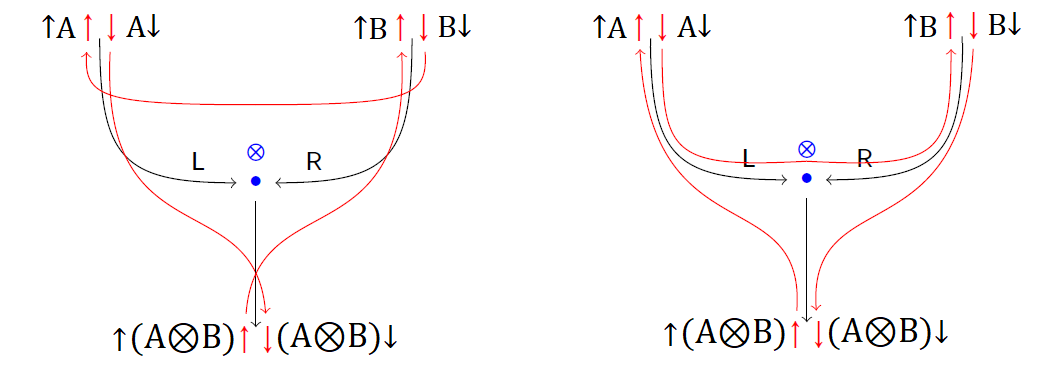
\includegraphics[width = 0.8\textwidth]{TensorSwitching.png}
    \caption{Tensor link, $L$ switching, $R$ switching}
    \label{fig:tensorswitching}
\end{figure}
\begin{figure}[h]
    \centering
    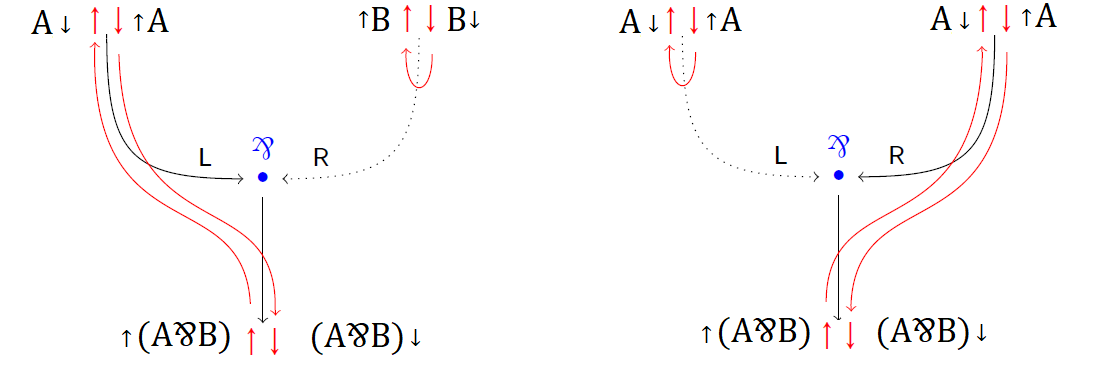
\includegraphics[width = 0.8\textwidth]{ParrSwitching.png}
    \caption{Par link, $L$ switching, $R$ switching.}
    \label{fig:parrswitching}
\end{figure}
\begin{defn}
Let $\operatorname{Pre}\call{T}(\pi,S)$ denote the set of all pretrips of $\pi$ with respect to $S$. We define an equivalence relation on this set $\sim$ where two pretrips $(x_1,...,x_n)$ and $(y_1,...,y_m)$ are equivalent if $n = m$, and there exists an integer $k$ such that $x_{i + k} = y_i$ (where $i + k$ means $\operatorname{mod} n$) for all $i = 1,...,n$.

A \textbf{trip} of $\pi$ with respect to $S$ is an equivalence class of pretrips. We denote the set of all trips by $\call{T}(\pi,S)$.  If the set $\call{T}(\pi,S)$ admits more than one element, these elements are called \textbf{short trips}, and if it admits only one element, this element is the \textbf{long trip}. We refer to the statement ``for all switchings $S$, the set $\call{T}(\pi,S)$ contains exactly one element" as the \textbf{long trip condition}.

A \textbf{short pretrip} is a choice of representative for a pretrip, and a \textbf{long pretrip} is a choice of representatitive of a long trip.
\end{defn}

\end{defn}
Given a proof-structure $\pi$ satisfying the long trip condition and a tensor link $\tau := (A,i,B,j, A \otimes B,k)$ of $\pi$, let $S$ be a switching of $\pi$ and $t := (x_1,...,x_n)$ be the long pretrip of $\pi$ satisfying $x_1 =A\downarrow$. Since $\pi$ satisfies the long trip condition, it must be the case that $\uparrow (A \otimes B)$ and $B\downarrow$ occur somewhere in $t$, can we determine which occurs earlier? Let $m,l > 0$ be such that $x_m = \uparrow (A \otimes B), x_l = B\downarrow$ and assume $l < m$. Say $S(\tau) = L$, then $t$ has the shape
\begin{equation}\label{eq:sequence_left_switch_tensor}
    (A\downarrow, (A \otimes B)\downarrow, ..., B \downarrow, \uparrow A, ..., \uparrow (A \otimes B), \uparrow B, ..., A\downarrow)
\end{equation}
Now consider the switching given by
\[\hat{S}(\sigma) = \begin{cases}
S(\sigma),& \sigma \neq \tau\\
R, & \sigma = \tau
\end{cases}
\]
Then \eqref{eq:sequence_left_switch_tensor} becomes:
\begin{equation}
    (A\downarrow, \uparrow B, ..., A\downarrow)
\end{equation}
which is a short pretrip, contradicting the assumption that $\pi$ satisfies the long trip condition. Thus $m < l$. We have proven (the first half) of:
\begin{lemma}\label{lem:stays_contained_tensor}
Let $\pi$ be a proof-structure satisfying the long trip condition, $\tau := (A,i,B,j, A \otimes B,k)$ be a tensor link of $\pi$, $S$ be a switching of $\pi$ and $(x_1,...,x_n)$ the long pretrip satisfying $x_1 = A \downarrow$. If $m,l > 0$ are such that $x_m = \uparrow (A \otimes B), x_l = B \downarrow$, then
\begin{itemize}
    \item if $S(\tau) = L$ then $m < l$,
    \item if $S(\tau) = R$ then $l < m$
\end{itemize}
\end{lemma}
The proof of the other half is similar to what has already been written, however since Lemma \ref{lem:stays_contained_tensor} contradicts \cite[Lemma 2.9.1]{linearlogic} we write out the details here:
\begin{proof}
Say $m < l$, then $t$ has the shape
\begin{equation}\label{eq:sequence_right_switch_tensor}
(A\downarrow, \uparrow B, ..., \uparrow (A \otimes B), \uparrow A, ..., B \downarrow, (A \otimes B)\downarrow, ..., A\downarrow)
\end{equation}
Now consider the switching given by
\[
S'(\sigma) = 
\begin{cases}
S(\sigma),& \sigma \neq \tau\\
L, & \sigma = \tau
\end{cases}
\]
Then \eqref{eq:sequence_right_switch_tensor} becomes:
\begin{equation}
    (A\downarrow, (A \otimes B)\downarrow,..., A\downarrow)
\end{equation}
which is a short pretrip.
\end{proof}
\begin{lemma}\label{lem:stays_contained_par}
Let $\pi$ be a proof-structure satisfying the long trip condition, $\tau := (A,i,B,i,A\parr B, k)$ be a par link of $\pi$, $S$ be a switching of $\pi$ and $(x_1,...,x_n)$ be the long pretrip satisfying $x_1 = A\downarrow$. If $m,l > 0$ are such that $x_m = \uparrow (A \parr B), x_l = B\downarrow$, then
\begin{itemize}
    \item if $S(\tau) = L$ then $m < l$,
    \item if $S(\tau) = R$ then $l < m$
\end{itemize}
\end{lemma}
\begin{proof}
Exercise.
\end{proof}
\begin{remark}
A long pretrip starting at position $1$ of Figure \ref{fig:stays_contained_explained_tens} necessarily moves to $1'$, granted the switching of the displayed tensor link is $L$. The long pretrip will necessarily return to this link, and moreover it will do so for the first time after leaving $1'$ either at position $2$ or $3$ (position $1$ will lead to a short trip). Lemma \ref{lem:stays_contained_tensor} states that in fact position $2$ will be taken next, then position $3$ at a later point. A similar story rings true if the switching is $R$.
\begin{figure}[h]
    \centering
    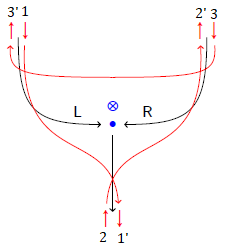
\includegraphics{TensorLeftSwitching.png}
    \caption{Left switching}
    \label{fig:stays_contained_explained_tens}
\end{figure}
This gives a nice interpretation of Lemma \ref{lem:stays_contained_tensor} that long trips \emph{return to where they left} at each tensor link.

The situation is a bit different for par links; we visit the premises before returning to the conclusion, see Figure \ref{fig:stays_contained_explained_par}.
\begin{figure}[h]
    \centering
    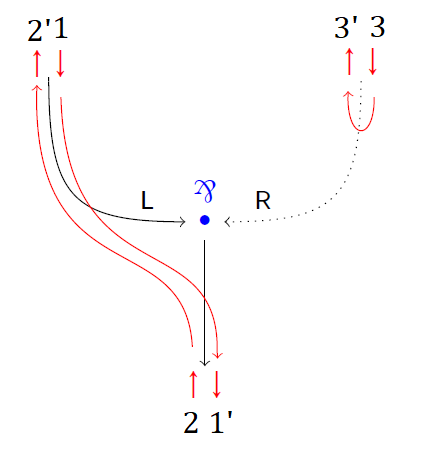
\includegraphics[width = 7cm]{ParLeftSwitching.png}
    \caption{Left switching}
    \label{fig:stays_contained_explained_par}
\end{figure}
\end{remark}
Loosely speaking, for a proof-structure $\pi$ satisfying the long trip condition to ``split" at a tensor link $\tau := (A,i,B,j,A\otimes B,k)$ into two distinct proof-structures $\pi_1,\pi_2$ each satisfying the long trip condition, it would necessarily be the case that any pretrip $\sigma$ of $\pi$ starting at $\uparrow A$ visits the entirety of $\call{U}(\pi_1)$ before returning to the tensor link $\tau$, lest $\pi_1$ admit a short trip. Moreover, it must be the case that $\sigma$ admits no occurrence of formulas in $\pi_2$ lest the result of removing the tensor link $\tau$ not result in disjoint proof-structures. Thus, if such a link $\tau$ exists, it is \emph{maximal} in the sense that there is no other tensor link $\tau' := (A',i',B',j',A' \otimes B',k')$ where a pretrip starting at $A'$ contains the entirety of any pretrip starting at $A$. The remainder of this Section will amount to proving the converse, that any such maximal tensor link ``splits" $\pi$.
\begin{defn}\label{def:pretrip_from_A}
Let $\pi$ be a proof-structure satisfying the long trip condition, $S$ a switching of $\pi$, and $A$ an occurrence of a formula in $\pi$. Consider the long pretrip $(x_1,...,x_n)$ satisfying $x_1 = \uparrow A$. We denote by
\begin{equation}
    \operatorname{PTrip}(\pi,S,A,\uparrow)
\end{equation}
the subsequence $(x_1,...,x_m)$ of $(x_1,...,x_n)$ satisfying $x_m = A\downarrow$. We define
\begin{equation}
    \operatorname{PTrip}(\pi, S, A, \downarrow)
\end{equation}
similarly.

Also, for $a \in \lbrace \uparrow,\downarrow\rbrace $ we define the following set
\begin{equation}
    \operatorname{Visit}_S(A,a) := \lbrace C \in \call{O}(\pi) \mid \uparrow C, C\downarrow \text{ occur in } \operatorname{PTrip}(\pi,S,A,a)\rbrace
\end{equation}
The \textbf{up empire of $A$} is the following set:
\begin{equation}
    \operatorname{Emp}_{\uparrow}A := \lbrace C \in \call{O}(\pi) \mid \text{For all switchings }S\text{ we have } \uparrow C, C\downarrow \text{ occur in } \operatorname{PTrip}(\pi,S, A,\uparrow)\rbrace
\end{equation}
The \textbf{down empire of $A$} is defined symmetrically.
\end{defn}
\begin{lemma}
for any formula $A$ which is a premise to either a tensor or par link, we have: $$\uparrow C \text{ occurs in } \operatorname{PTrip}(\pi,S,A,\uparrow)\qquad\text{ if and only if }\qquad C\downarrow \text{ occurs in } \operatorname{PTrip}(\pi,S,A,\uparrow)$$
\end{lemma}
\begin{defn}
The \textbf{complexity} of a preformula $A$ is the sum of the number of occurrences of $\otimes$ and the number of occurrences of $\parr$ which appear in $A$. Notice that this number is invariant under choice of representative for a formula and so we also have the \textbf{complexity} of a formula.
\end{defn}
\begin{proof}
For simplicity we denote $\operatorname{PTrip}(\pi, S, A, a)$ by $\operatorname{PTrip}(A, a)$.

We proceed by induction on the \emph{complexity} of $A$ denoted $c(A)$. Say $A$ is atomic so that $c(A) = 0$. Then $A$ is part of an axiom link and
\begin{equation}
    \operatorname{PTrip(A,\uparrow)} = \uparrow A, \operatorname{PTrip}(\negation A, \downarrow), A\downarrow
\end{equation}
If $\negation A$ is a conclusion then we have $C = \negation A$ and we are done.

If $\negation A$ is a premise to a tensor link
\end{proof}

With this new terminology we now have some corollaries of Lemmas \ref{lem:stays_contained_tensor} and \ref{lem:stays_contained_par}:
\begin{cor}\label{cor:pretrip_innards}
Let $\pi$ be a proof-structure satisfying the long trip condition, and let $S$ be a switching of $\pi$, for a formula $A$ and $a \in \lbrace \uparrow, \downarrow\rbrace$, denote $\operatorname{PTrip}(\pi,S, A, a)$ by $\operatorname{PTrip}(A,a)$:
\begin{enumerate}
    \item if $A$ is part of an axiom link then
    \begin{equation}
        \operatorname{PTrip}(A,\uparrow) = \uparrow A, \operatorname{PTrip}(\negation A, \downarrow), A \downarrow
    \end{equation}
    \item if $\tau$ is a tensor link with conclusion $A \otimes B$:
    \begin{enumerate}
        \item if $S(\tau) = L$:
    \begin{equation}
        \operatorname{Ptrip}(A, \downarrow) = A\downarrow, \operatorname{PTrip}(A \otimes B, \downarrow), \operatorname{PTrip}(B, \uparrow), \uparrow A
    \end{equation}
    \begin{equation}
        \operatorname{PTrip}(B, \downarrow) = B\downarrow, \operatorname{PTrip}(A,\uparrow), \operatorname{PTrip}(A \otimes B, \downarrow), \uparrow B
    \end{equation}
    \begin{equation}
        \operatorname{PTrip}(A \otimes B, \uparrow) = \uparrow A \otimes B, \operatorname{PTrip}(B, \uparrow), \operatorname{PTrip}(A,\uparrow), A \otimes B \downarrow
    \end{equation}
        \item if $S(\tau) = R$:
    \begin{equation}
        \operatorname{PTrip}(A, \downarrow) = A\downarrow, \operatorname{PTrip}(B, \uparrow),\operatorname{PTrip}(A \otimes B, \downarrow), \uparrow A
    \end{equation}
    \begin{equation}
        \operatorname{PTrip}(B, \downarrow) = B\downarrow,  \operatorname{PTrip}(A \otimes B, \downarrow), \operatorname{PTrip}(A,\uparrow),\uparrow B
    \end{equation}
    \begin{equation}
        \operatorname{PTrip}(A \otimes B, \uparrow) = \uparrow A \otimes B,  \operatorname{PTrip}(A,\uparrow), \operatorname{PTrip}(B, \uparrow),A \otimes B \downarrow
    \end{equation}
    \end{enumerate}
    \item if $A$ is a premise of a par link $\tau$ with conclusion $A \parr B$:
    \begin{enumerate}
        \item if $S(\tau) = L$:
        \begin{equation}
            \operatorname{PTrip}(A,\downarrow) = A\downarrow, \operatorname{PTrip}(A \parr B, \downarrow), \uparrow A
        \end{equation}
        \begin{equation}
            \operatorname{PTrip}(B, \downarrow) = B\downarrow, \uparrow B
        \end{equation}
        \begin{equation}
            \operatorname{PTrip}(A \parr B, \uparrow) = \uparrow A \parr B, \operatorname{PTrip}(A, \uparrow), A \parr B \downarrow
        \end{equation}
        \item if $S(\tau) = R$:
        \begin{equation}
            \operatorname{PTrip}(A,\downarrow) = A\downarrow, \uparrow A
        \end{equation}
        \begin{equation}
            \operatorname{PTrip}(B, \downarrow) = B\downarrow, \operatorname{PTrip}(A \parr B, \downarrow), \uparrow B
        \end{equation}
        \begin{equation}
            \operatorname{PTrip}(A \parr B, \uparrow) = \uparrow A \parr B, \operatorname{PTrip}(B, \uparrow), A \parr B \downarrow
        \end{equation}
    \end{enumerate}
\end{enumerate}
\end{cor}
In particular:
\begin{cor}\label{cor:stays_contained_corollary}
For any formula $A$ which is a premise to either a tensor or par link, and any $a \in \lbrace \uparrow, \downarrow \rbrace$, we have: $$\uparrow C \text{ occurs in } \operatorname{PTrip}(\pi,S,A,\uparrow)\qquad\text{ if and only if }\qquad C\downarrow \text{ occurs in } \operatorname{PTrip}(\pi,S,A,\downarrow)$$ and similarly for $\operatorname{PTrip}(\pi,S,A,\downarrow)$.
\end{cor}
\begin{proof}
By induction on the length of the sequence $\operatorname{PTrip}(\pi,S,A,a)$ and appealing to Corollary \ref{cor:pretrip_innards}.
\end{proof}
\begin{cor}\label{cor:empire_features}
Let $\pi$ be a proof-structure satisfying the long trip condition,
we have:
\begin{enumerate}
    \item\label{cor:empire_features_up_ax} for any axiom link with conclusions $A, \negation A$:
    \begin{equation}
        \operatorname{Emp}_{\uparrow}A = \operatorname{Emp}_{\downarrow}(\negation A) \cup \lbrace A \rbrace
    \end{equation}
    \item\label{cor:empire_features_down_cut} for any cut link with premises $A, \negation A$:
    \begin{equation}
        \operatorname{Emp}_{\downarrow}A = \operatorname{Emp}_{\uparrow}(\negation A) \cup \lbrace A \rbrace
    \end{equation}
    \item\label{cor:empire_features_empty_int} for any tensor link with premises $A,B$:
    \begin{equation}
        \operatorname{Emp}_{\uparrow}A \cap \operatorname{Emp}_{\uparrow}B = \varnothing
    \end{equation}
    \item\label{cor:empire_features_up_tens_par} for any tensor or par link with premises $A,B$ and conclusion $C$:
    \begin{equation}
        \operatorname{Emp}_{\uparrow}C = \operatorname{Emp}_{\uparrow}A \cup \operatorname{Emp}_{\uparrow}B \cup \lbrace C \rbrace
    \end{equation}
    \item\label{cor:empire_features_down_tens} for any tensor link with premises $A,B$:
    \begin{equation}
        \operatorname{Emp}_{\downarrow}B = \operatorname{Emp}_{\uparrow}A \cup \operatorname{Emp}_{\downarrow}(A \otimes B) \cup \lbrace B \rbrace
    \end{equation}
    and similarly,
    \begin{equation}
        \operatorname{Emp}_{\downarrow}A = \operatorname{Emp}_{\uparrow}B \cup \operatorname{Emp}_{\downarrow}(A \otimes B) \cup \lbrace A\rbrace
    \end{equation}
\end{enumerate}
\end{cor}
\begin{remark}
Recall Definition \ref{def:proof_structures} that there are two types of tensor links $(A,i,B,j,A\otimes B,k)$,
$(B,j,A,i,A\otimes B,k)$ and two types of par links $(A,i,B,j,A\parr B, k),(B,j,A,i,A\parr B,k)$. Lemmas \ref{lem:stays_contained_tensor} and \ref{lem:stays_contained_par} were only stated for links of the form $(A,i,B,j,A\otimes B,k), (A,i,B,j,A\parr B, k)$ however they hold for \emph{all} tensor and par links. One merely replaces all instances of $A \otimes B$ with $B \otimes A$, and all instances of $A \parr B$ with $B \parr A$ in the proofs.
\end{remark}
\begin{defn}
Given any link $\tau$ we write $B \in \tau$ if $B$ occurs as either a premise or a conclusion of $\tau$.

Let $\pi$ be a proof-structure satisfying the long trip condition, and $a \in \lbrace \uparrow, \downarrow\rbrace$. The set of \textbf{links of $A$ with respect to $S$} is the set
\begin{equation}
    \operatorname{Link}_aA := \lbrace \tau \in \operatorname{Link}\pi \mid \forall B \in \tau, B \in \operatorname{Emp}_aA \rbrace
\end{equation}
\end{defn}
\begin{defn}
Let $\pi$ be a proof-structure satisfying the long trip condition and let $a \in \lbrace \uparrow, \downarrow \rbrace$. Define the set
\begin{equation}
    \operatorname{Link}^0_{\parr,a}A := \lbrace \tau \in \operatorname{Link}\pi \mid \text{Exactly one premise of }\tau\text{ is in }\operatorname{Emp}_{a}A\rbrace
\end{equation}
\end{defn}
\begin{lemma}[Realisation Lemma]\label{lem:realisation_switching}
Let $\pi$ be a cut-free proof-structure satisfying the long trip condition, let $a \in \lbrace \uparrow, \downarrow \rbrace$ and $A$ an occurrence of a formula in $\pi$. Define the following function:
\begin{align*}
    S: \operatorname{Link}_{\parr,a}^0A &\lto \lbrace L,R\rbrace\\
    \tau &\longmapsto
    \begin{cases}
    L, & \text{if the right premise of }\tau\text{ is in }\operatorname{Emp}_{a}A\\
    R, & \text{if the left premise of }\tau\text{ is in }\operatorname{Emp}_{a}A
    \end{cases}
\end{align*}
and extend this to a switching $\hat{S}: \operatorname{Link}\pi \lto \lbrace L,R \rbrace$ arbitrarily. Then
\begin{equation}
    \operatorname{Emp}_aA = \operatorname{Visit}_{\hat{S}}(A,a)
\end{equation}
\end{lemma}
\begin{proof}
We proceed by induction on the size $|\operatorname{Link}_a(A)|$ of the set $\operatorname{Link}_a(A)$. For the base case, assume $|\operatorname{Link}_a(A)| = 0$. The formula $A$ is part of an axiom link and so $\operatorname{Emp}_{\uparrow}A = A, \negation A$ and $\operatorname{Emp}_{\downarrow}A = A$, the result follows easily.

Now assume that $|\operatorname{Link}_a A| = n > 0$ and the result holds for any formula $B$ such that $|\operatorname{Link}_aB| < n$. First say $a = \uparrow$, and $A$ is a conclusion of either a tensor or a par link
\[
\begin{tikzcd}[column sep = tiny]
A_1\arrow[dr,dash] && \negation A_2\arrow[dl,dash]\\
& A
\end{tikzcd}
\]
where $A = A_1 \otimes A_2$ or $A = A_1 \parr A_2$. By \eqref{cor:empire_features_up_tens_par} we have
\begin{align*}
    \operatorname{Emp}_{\uparrow}A &= \operatorname{Emp}_{\uparrow}A_1 \cup \operatorname{Emp}_{\uparrow}A_2 \cup \lbrace A\rbrace\\
    &= \operatorname{Visit}_{\hat{S}}(A_1,\uparrow) \cup \operatorname{Visit}_S(A_2,\uparrow) \cup \lbrace A \rbrace\\
    &= \operatorname{Visit}_{\hat{S}}(A, \uparrow)
\end{align*}
where the second equality follows from the inductive hypothesis.

Assume $A$ is part of an axiom link. By \eqref{cor:empire_features_up_ax}
\begin{equation}
    \operatorname{Emp}_{\uparrow}A = \operatorname{Emp}_{\downarrow}(\negation A) \cup \lbrace A \rbrace
\end{equation}
with
\begin{equation}
    |\operatorname{Link}_{\uparrow}A| = |\operatorname{Link}_{\downarrow}(\negation A)|
\end{equation}
Since $|\operatorname{Link}_{\downarrow}(\negation A)| > 0$ we necessarily have that $\negation A$ is not a conclusion. Thus, since $\pi$ is cut-free, $A$ is connected to an occurrence $\negation A$ which is a premise to either a tensor link or a par link. In the case of the former, we have:
\[
\begin{tikzcd}[column sep = tiny]
C\arrow[dr,dash] && \negation A\arrow[dl,dash]\\
& C \otimes \negation A
\end{tikzcd}
\]
then by \eqref{cor:empire_features_down_tens}:
\begin{align*}
    \operatorname{Emp}_{\downarrow}(\negation A) &= \operatorname{Emp}_{\uparrow}C \cup \operatorname{Emp}_{\downarrow}(C \otimes \negation A) \cup \lbrace \negation A\rbrace\\
    &= \operatorname{Visit}_{\hat{S}}(C,\uparrow) \cup \operatorname{Visit}_{\hat{S}}(C \otimes \negation A,\downarrow) \cup \lbrace \negation A\rbrace\\
    &= \operatorname{Visit}_{\hat{S}}(\negation A, \downarrow)
\end{align*}
where the second equality follows from the inductive hypothesis.

If $\negation A$ is a premise of a par link
\[
\begin{tikzcd}[column sep = tiny]
C\arrow[dr,dash] && \negation A\arrow[dl,dash]\\
& C \parr \negation A
\end{tikzcd}
\]
then by construction of $\hat{S}$, where we use the specific definition of $S$ for the first time,
\begin{align*}
    \operatorname{Emp}_{\downarrow}(\negation A) &= \lbrace \negation A\rbrace\\
    &= \operatorname{Visit}_{\hat{S}}(\negation A,\downarrow)
\end{align*}
The case when $a = \downarrow$ is exactly similar and so we omit the proof.
\end{proof}
\begin{defn}
A tensor or par link is \textbf{terminal} if it is a conclusion.
\end{defn}
\begin{cor}\label{lem:par_link_existence}
Let $\pi$ be a cut-free proof-structure satisfying the long trip condition. Let
\[
\tau := \begin{tikzcd}[column sep = tiny]
A\arrow[dr,dash] && B\arrow[dl,dash]\\
& A \otimes B
\end{tikzcd}
\]
be a terminal tensor link of $\pi$. Then $\pi$ admits a par link
\[
\sigma := \begin{tikzcd}[column sep = tiny]
C\arrow[dr,dash] && D\arrow[dl,dash]\\
& C \parr D
\end{tikzcd}
\]
such that either $C \in \operatorname{Emp}_{\uparrow}A$ and $D \in \operatorname{Emp}_{\uparrow}B$ or $C \in \operatorname{Emp}_{\uparrow}B$ and $D \in \operatorname{Emp}_{\uparrow}A$ if and only if for any switching $S$ of $\pi$ we have that either
\[\operatorname{Emp}_{\uparrow}A \subsetneq \operatorname{Visit}_S(A,\uparrow)\qquad\text{or}\qquad \operatorname{Emp}_{\uparrow}B \subsetneq \operatorname{Visit}_S(B,\uparrow)\]
\end{cor}
\begin{proof}
Say $\pi$ admitted $\sigma$ and $C \in \operatorname{Emp}_{\uparrow}A$ and $D \in \operatorname{Emp}_{\uparrow}B$. If the switching $S$ is such that $S(\tau) = L$ then $C \parr D \in \operatorname{Visit}_S(B)\setminus \operatorname{Emp}_{\uparrow}B$ and if $S(\tau) = R$ then $C \parr D \in \operatorname{Visit}_S(A) \setminus \operatorname{Emp}_{\uparrow}A$. The other case is similar.

Conversely, say $\pi$ admits no such par link $\sigma$, that is, assume
\begin{equation}
    \operatorname{Link}^0_{\parr,\uparrow}(A) \cap \operatorname{Link}^0_{\parr,\uparrow}(B) = \varnothing
\end{equation}
Then there is by Lemma \ref{lem:realisation_switching} a well defined function $$S: \operatorname{Link}_{\parr,\uparrow}^0(A) \cup \operatorname{Link}^0_{\parr,\uparrow}(B) \lto \lbrace L, R \rbrace$$ which extends to a switching $\hat{S}$ such that
\begin{equation}
    \operatorname{Emp}_{\uparrow}A = \operatorname{Visit}_{\hat{S}}(A,\uparrow)\qquad\text{and}\qquad \operatorname{Emp}_{\uparrow}B = \operatorname{Visit}_{\hat{S}}(B,\uparrow)
\end{equation}
\end{proof}

\begin{lemma}[Separation Lemma]
A cut-free proof-structure $\pi$ satisfying the long trip condition, with only tensor links amongst its conclusions admits a tensor link
\[
\tau := \begin{tikzcd}[column sep = tiny]
A\arrow[dr,dash] && B\arrow[dl,dash]\\
& A \otimes B
\end{tikzcd}
\]
satisfying
\begin{equation}
    \call{O}(\pi) = \operatorname{Emp}_{\uparrow}A \cup \operatorname{Emp}_{\uparrow}B \cup \lbrace A \otimes B\rbrace
\end{equation}
Moreover, removing $A \otimes B$ results in a disconnected graph with each component a proof-structure satisfying the long trip condition.
\end{lemma}
\begin{proof}
Consider the set of tensor links $\operatorname{Link}_{\otimes}(\pi)$ of $\pi$. We endow this with the following partial order $\leq$: a pair of links:
\[
\sigma := 
\begin{tikzcd}[column sep = tiny]
A\arrow[dr,dash] && B\arrow[dl,dash]\\
& A \otimes B
\end{tikzcd}
%
\qquad
%
\rho :=
\begin{tikzcd}[column sep = tiny]
C\arrow[dr,dash] && D\arrow[dl,dash]\\
& C \otimes D
\end{tikzcd}
\]
are such that $\tau \leq \sigma$ if $\operatorname{Emp}_{\uparrow}A \cup \operatorname{Emp}_{\uparrow}B \subseteq \operatorname{Emp}_{\uparrow}C \cup \operatorname{Emp}_{\uparrow}D$. Let $\tau$ (with conclusion $A \otimes B$ say) be a tensor link maximal with respect to $\leq$. We show that $\tau$ satisfies the required property.

Say $\call{O}(\pi) \neq \operatorname{Emp}_{\uparrow}A \cup \operatorname{Emp}_{\uparrow}B \cup \lbrace A \otimes B\rbrace$. Then by Lemma \ref{lem:par_link_existence} there exists a par link
\[
\sigma := \begin{tikzcd}[column sep = tiny]
C\arrow[dr,dash] && D\arrow[dl,dash]\\
& C \parr D
\end{tikzcd}
\]
such that either $C \in \operatorname{Emp}_{\uparrow}A$ and $D \in \operatorname{Emp}_{\uparrow}B$ or $C \in \operatorname{Emp}_{\uparrow}B$ and $D \in \operatorname{Emp}_{\uparrow}A$. We show the proof in the case of the former. Since $\pi$ admits no terminal par links, this link is above a tensor link
\[
\rho := \begin{tikzcd}[column sep = tiny]
E\arrow[dr,dash] && F\arrow[dl,dash]\\
& E \otimes F
\end{tikzcd}
\]
Notice that if $\rho = \tau$, then either $C \parr D \in \operatorname{Emp}_{\uparrow}A$ or $C \parr D \in \operatorname{Emp}_{\uparrow}B$ which in either case implies $\operatorname{Emp}_{\uparrow}A \cap \operatorname{Emp}_{\uparrow}B \neq \varnothing$, contradicting Corollary \ref{cor:empire_features}, \ref{cor:empire_features_empty_int}, and so $\rho \neq \tau$. Without any loss of generality, assume that $\sigma$ sits above $F$. Let $S$ be a switching of $\pi$ so that $\operatorname{Emp}_{\uparrow}F = \operatorname{Visit}_S(F,\uparrow)$ and so that $S(\sigma) = L$, which exists by Lemma \ref{lem:par_link_existence}. Let $t = (x_1,...,x_n)$ be the long pretrip of $\pi$ with respect to $S$ satisfying $x_1 = F\uparrow$. We have by Lemma \ref{lem:stays_contained_par} that $t$ takes the following shape:
\begin{equation}\label{eq:condemning_shape}
    \uparrow F, ..., \uparrow(C \parr D), \uparrow C, ..., D\downarrow, \uparrow D, ..., C\downarrow, (C \parr D)\downarrow, ..., F\downarrow,...
\end{equation}
We have that $D \in \operatorname{Emp}_{\uparrow}B$ so for simplicity, rewrite \eqref{eq:condemning_shape} as $t' = (x_{1 + k},...,x_{n+k})$ for some $k > 0$ (where $i + k$ means $i + k\operatorname{mod} n$) so that $t$ takes the shape
\begin{equation}\label{eq:condemning_shape_altered}
     ..., \uparrow F, ..., \uparrow(C \parr D), \uparrow C, ..., D\downarrow, \uparrow D, ..., C\downarrow, (C \parr D)\downarrow, ..., F\downarrow,...
\end{equation}
with $\uparrow B$ occurring to the left of $D \downarrow$ and $B \downarrow$ occurring to the right of $\uparrow D$.
We have that $C \not\in \operatorname{Emp}_{\uparrow}B$ and so by Corollary \ref{cor:stays_contained_corollary}:
\begin{equation}
\uparrow B \text{ occurrs in }\uparrow C,..., D\downarrow\text{ and } B\downarrow\text{ occurrs in }\uparrow D, ..., C\downarrow
\end{equation}
However, this implies that $B \in \operatorname{Visit}_S(F,\uparrow)$ which by Lemma \ref{lem:realisation_switching} implies $B \in \operatorname{Emp}_{\uparrow}F$.

By reversing the switching of $\sigma$ and interchanging the rolls of $C,D$ in the above argument, we also have that $A \in \operatorname{Emp}_{\uparrow}F$, contradicting the maximality of $\tau$. This proves the first claim.

For the second claim, since $\call{O}(\pi) = \operatorname{Emp}_{\uparrow}A \cup \operatorname{Emp}_{\uparrow}B \cup \lbrace A \otimes B\rbrace$ we have by Lemma \ref{lem:par_link_existence} that
\begin{equation}
    \operatorname{Link}_{\parr,\uparrow}^0(A\otimes B) = \varnothing
\end{equation}
and we saw in the proof of Lemma \ref{lem:realisation_switching} that a switching $S$ which realises $\operatorname{Emp}_{\uparrow}A$ is given by setting all switchings arbitrarily except for those in $\operatorname{Link}_{\parr,\uparrow}^0(A\otimes B)$. This means that for any switching $S$ of $\pi$:
\begin{equation}
    \operatorname{Visit}_{S}(A,\uparrow) = \operatorname{Emp}_{\uparrow}A \qquad\text{and}\qquad \operatorname{Visit}_{S}(B,\uparrow) = \operatorname{Emp}_{\uparrow}B
\end{equation}
which is to say the two subproof-structures given by removing $A \otimes B$ never admit a short trip, that is, they each satisfy the long trip condition.
\end{proof}
\begin{thm}[The Sequentialisation Theorem]\label{thm:sequentialisation}
A proof-structure $\pi$ (possibly with cuts) satisfies the long trip condition if and only $\pi$ is a proof-net.
\end{thm}
\begin{proof}
First assume that $\pi$ is cut-free.

We proceed by induction on the size $|\operatorname{Link}\pi|$ of the set $\operatorname{Link}\pi$. If there this is zero then $\pi$ consists of a single axiom link and so the result is clear.

For the inductive step, we consider two cases, first say $\pi$ admits a par link for a conclusion. Then removing this par link clearly results in two cut-free subproof-structures satsifying the long trip condition and so the result follows from the inductive hypothesis. If no such terminal par link exists, then by the Separation Lemma there exists some tensor link in the conclusion for which we can remove and apply the inductive hypothesis.

Now say that $\pi$ contained cuts. We replace each cut with a tensor link to create a new proof $\zeta$. That there exists a proof $\Xi$ which maps to $\zeta$ follows from the part of the result proved already as $\zeta$ is cut-free. We adapt $\Xi$ appropriately by replacing $\otimes$-rules by $\operatorname{cut}$-rules and we are done.
\end{proof}
\section{Cut}
The cut-reduction process may involve re-writing vertex labels. For this we introduce the following substitution operation:
\begin{defn}[Labelled formula substitution]
Given a labelled formula $x_1: A_1 \boxtimes_{1} \hdots \boxtimes_{n-1} x_n: A_n$, where each $\boxtimes_i \in \lbrace \otimes, \parr \rbrace$, we denote by
\begin{equation}\label{eq:labelled_form_substitution}
(x_1: A_1 \boxtimes_{1} \hdots \boxtimes_{n-1} x_n: A_n)[x_i := y_i]
\end{equation}
the labelled formula given by replacing every instance of $x_i$ in $x_1: A_1 \boxtimes_{1} \hdots \boxtimes_{n-1} x_n: A_n$ by $y_i$. To avoid clutter, we continue the convention of not writing the labels, and so \eqref{eq:labelled_form_substitution} may just as well be written $A[x_i := y_i]$, where $A$ denotes $x_1: A_1 \boxtimes_{1} \hdots \boxtimes_{n-1} x_n: A_n$.
\end{defn}
\begin{defn}\label{def:proof_structure_parts}
A \textbf{proof-structure part} is a subgraph of proof-structures which need not be a proof-structure itself.
\end{defn}
\begin{defn}[Proof substitution]
Given a proof structure $\pi$, we denote by $\pi[x:=y]$ the proof structure given by replacing every labelled formula $A$ in $\pi$ by $A[x_i := y_i]$. Similarly, we define substitution on proof-structure parts. 
\end{defn}
\begin{defn}\label{def:cut_reduction}[Cut-reduction]
Cut-reduction $\lto_{\operatorname{cut}}$ is the smallest, compatible equivalence relation on the set of all proof-nets containing the following generators (for clarity, the occurrence labels have been written in explicitly):
\begin{itemize}
    \item \textbf{Axiom redex} Consider a proof-structure $\pi$ of the following shape:
    \begin{equation}\label{eq:cut_red_ax}
    \begin{tikzcd}[column sep = tiny]
    & & \pi_1\arrow[d,dash]\\
        x:A\arrow[r,dash, bend left]\arrow[d,dash] & y:\negation A\arrow[r,dash, bend right] & z:A\\
        \pi_2
    \end{tikzcd}
\end{equation}
with $\pi_1,\pi_2$ possibly connected proof-structure parts. We first consider the proof-structure part given by removing $y:\negation A$ (and the incident edges) from \eqref{eq:cut_red_ax},  denote this $\zeta$. We then construct $\zeta[z := x]$ and then identify the displayed occurrences of $x:A, z:A$ which due to the substitution are now both $x:A$. The result is a proof-structure $\pi'$, this is the image of $\pi$ under cut-reduction in this case.
    \item \textbf{Tensor-par redex}
       \begin{equation}\label{eq:cut_red_tens}
        \begin{tikzcd}[column sep = tiny]
            A\arrow[dr,dash] && B\arrow[dl,dash] & \negation A\arrow[dr,dash] && \negation B\arrow[dl,dash]\\
            & A \otimes B\arrow[rrr,dash, bend right] & & & \negation A \parr \negation B
        \end{tikzcd}
    \end{equation}
    $\lto_{\operatorname{cut}}$
    \begin{equation}
    \begin{tikzcd}
        (A,i)\arrow[rr,dash,bend right] & (B,j)\arrow[rr,dash,bend right] & (\negation A, k) & (\negation B, l)
        \end{tikzcd}
    \end{equation}
\end{itemize}
The reflexive, symmetric, transitive closure of cut-reduction is \textbf{cut-equivalence}, and is denoted $\sim_{\operatorname{cut}}$.

A pair consisting of an axiom link and a cut link in the shape of \eqref{eq:cut_red_ax} is a \textbf{axiom redex}, and a set consisting of occurrences of formulas, a tensor link, a par link, and a cut link in the shape of \eqref{eq:cut_red_tens} is a \textbf{tensor-par redex}.
\end{defn}
\begin{proposition}[Church-Rosser]\label{prop:church_rosser}
If $\pi_1$ is a proof-structure and $\pi_1 \lto_{\operatorname{cut}} \pi_2, \pi_1 \lto_{\operatorname{cut}} \pi_3$ then there exists a proof-structure $\pi_4$ such that $\pi_2 \lto_{\operatorname{cut}} \pi_4, \pi_3 \lto_{\operatorname{cut}} \pi_4$.
\end{proposition}
\begin{proof}
The key observation is that reducing any redex in a proof does not eliminate any other redex.
\end{proof}
\begin{defn}\label{def:permutations}
Let $\pi$ be a proof-net with $n$ axiom links. Assume the occurrences of the axioms of $\pi$ have been labelled by integers $1,...,2n$. For each $1 \leq m \leq 2n$ let $\alpha_{\pi}(m)$ denote the integer such that the formulas labelled $m,\alpha_{\pi}(m)$ are connected by an axiom link in $\pi$. This defines a permutation (which is a disjoint union of transpositions) which we call the \textbf{axiom link permutation associated to $\pi$}.

There is another permutation of $\lbrace 1,...,2n\rbrace$ defined by $\pi$. Let $S$ be a switching of $\pi$ and for each $1 \leq m \leq 2n$ let $\beta_{\pi}^S(m)$ denote the integer such that the first occurrence of any $\uparrow A_1,...,\uparrow A_{2n}$ in $\operatorname{PTrip}(\pi,S,A_m,\downarrow)$ (Definition \ref{def:pretrip_from_A}) is $\uparrow A_{\beta_{\pi}(m)}$.

The set of all premutations of the second form is denoted:
\begin{equation}
    \Sigma(\pi) := \lbrace \beta_{\pi}^S \mid S\text{ is a switching of }\pi\rbrace
\end{equation}
We will often denote elements of $\beta_{\pi}^S \in \Sigma(\pi)$ simply by $\beta$.
\end{defn}
\begin{remark}
A provable formula $A$ uniquely defines a cut-free proof-structure with soul conclusion $A$ up to the axiom links. For instance, the formula 
\begin{equation}
(A \otimes A) \parr (\negation A \parr \negation A)
\end{equation}
corresponds to the sub-proof-structure given by ignoring the dashed lines and the axiom links of \eqref{eq:counter_one}:
\begin{equation}\label{eq:counter_one}
\begin{tikzcd}[column sep = tiny]
A \arrow[rr,dash, bend left] \arrow[rd,dash]\arrow[rrrrrr,bend left,dash,dashed] &                         & \negation A \arrow[rr,dash,bend left, dashed] \arrow[rrrd,dash] &                                                     & A \arrow[rr,dash, bend left] \arrow[llld,dash] &                                           & \negation A \arrow[ld,dash] \\
                                   & A \otimes A \arrow[rrd,dash] &                        &                                                     &                                    & \negation A \parr \negation A \arrow[lld,dash] &                        \\
                                   &                         &                        & (A \otimes A) \parr (\negation A \parr \negation A) &                                    &                                           &                       
\end{tikzcd}
\end{equation}
The proof-net given by ignoring the dashed lines in \eqref{eq:counter_one} corresponds to the permutation $(12)(34)$, and that given by ignoring the axiom links and including the dashed lines is $(14)(23)$.

Note: in the notation of \cite{multiplicatives} this sub-proof structure would be denoted $T_{A'}$, where $A' = (A \otimes A) \parr (\negation A \parr \negation A)$.
\end{remark}
\begin{defn}
Let $\pi$ be a proof-net possibly containing cut links. A \textbf{reduction sequence} is a sequence
\begin{equation}
    \pi = \pi_0 \lto_{\operatorname{cut}} \pi_1 \lto_{\operatorname{cut}} \hdots \lto_{\operatorname{cut}} \pi_n
\end{equation}
with $\pi_n$ cut-free.
\end{defn}
\begin{lemma}\label{lem:red_sequence_existence}
Every proof-net $\pi$ admits a reduction sequence.
\end{lemma}
\begin{proof}
Given a cut link $\tau := (A,i,\negation A, j)$ in $\pi$, the \textbf{complexity of $\tau$}, $c(\tau)$ is the sum of the number of occurrences of $\otimes$ and the number of occurrences of $\parr$ in $A$. We proceed by induction on the maximum of the complexities of all cut links in $\pi$.

Say this maximum is $0$. Then all cut-links have the shape of \eqref{eq:cut_red_ax} (using the fact that $\pi$ is a \emph{proof-net}, not merely a proof-structure). We can use \eqref{eq:cut_red_ax} finitely many times (in any order) to deduce the result.

Now say the maximum is $n > 0$. We then apply \eqref{eq:cut_red_tens} to all cut links of complexity $n$ (in any order) to obtain a new proof-structure $\zeta$. It follows from Lemmas \ref{fig:stays_contained_explained_tens}, \ref{fig:stays_contained_explained_par} that $\pi$ satisfying the long trip condition ensures that $\zeta$ does, and so we may apply the inductive hypothesis.
\end{proof}
\begin{defn}
Let $\operatorname{Red}\pi$ denote the set of all reduction sequences of $\pi$. The \textbf{length} $l(\underline{x})$ of a reduction sequence $\underline{x} \in \operatorname{Red}\pi$ is the length of the sequence $\underline{x}$.
\end{defn}
\begin{cor}\label{cor:stable_length}
The length of a reduction path is independent of the choice of reduction path.
\end{cor}
\begin{proof}
The proof is purely geometric. Let
\begin{equation}
    \underline{x} := ( \pi = \pi_1 \lto_{\operatorname{cut}} \hdots \lto_{\operatorname{cut}} \pi_n)
\end{equation}
be the reduction path described by Lemma \ref{lem:red_sequence_existence} and let
\begin{equation}
    \underline{y} := (\pi = \zeta_0 \lto_{\operatorname{cut}} \hdots \lto_{\operatorname{cut}} \zeta_n)
\end{equation}
be any other reduction sequence. By Lemma \ref{prop:church_rosser} we have $\pi_n = \zeta_n$. Also using \ref{prop:church_rosser}, the pair of reduction paths can be completed to some grid defined by a subset of $\bb{N} \times \bb{N}$. All paths $p$ consisting of only upwards steps or right steps such that $p$ is bound to this grid have the same length and so $l(\underline{x}) = l(\underline{y})$.
\end{proof}
\begin{defn}\label{def:normal_form}
The proof of Corollary \ref{cor:stable_length} shows that every reduction path of a proof-net $\pi$ leads to the same cut-free proof $\zeta$. We call $\zeta$ the \textbf{normal form} of $\pi$.
\end{defn}
\begin{cor}
Multiplicative proof-nets are strongly normalising.
\end{cor}
\section{Orthogonality}









\begin{proposition}
Let $\pi$ be a proof-structure, then $\pi$ is a proof-net if and only if for all $\beta \in \Sigma(\pi)$ the permutation $\alpha_{\pi}\beta$ is cyclic.
\end{proposition}
\begin{lemma}\label{lem:pars_or_not}
Let $\pi$ be a proof-net with conclusions $A_1,...,A_n$ and let $\zeta$ be a proof-net obtained by beginning with $\pi$ and in any order forming par links which connect all the conclusions $A_1,...,A_n$ so that $\zeta$ has conclusions $B_1,...,B_m$ where $m \leq n$ and each $B_i$ is constructed only by $\parr$ and a subset of the formulas $A_1,...,A_n$. Then $\Sigma(\pi) = \Sigma(\zeta)$.
\end{lemma}
\begin{proof}
Easy proof by induction on the integer given by the number of par links in $\zeta$ minus the number of par links in $\pi$.
\end{proof}
\begin{example}\label{ex:counter}
\begin{figure}[h]
    \centering
    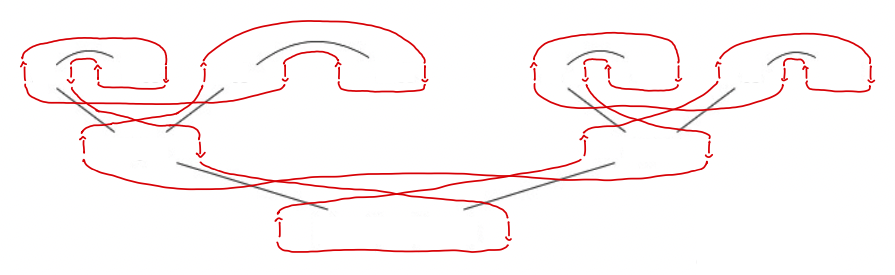
\includegraphics[width = 17cm]{Permutations.png}
    \caption{The set $\Sigma(\pi_1)$}
    \label{fig:counter_one}
\end{figure}
Let $\pi_1$ be as defined as follows:
\begin{equation}
\pi_1 = \begin{tikzcd}
A \arrow[r, dash,bend left] \arrow[rd,dash] & \negation A             & A \arrow[r, dash,bend left] \arrow[ld,dash] & \negation A                         & A \arrow[r, dash,bend left] \arrow[rd,dash] & \negation A             & A \arrow[r, dash,bend left] \arrow[ld,dash] & \negation A \\
                                  & A \otimes A \arrow[rrd,dash] &                                   &                                     &                                   & A \otimes A \arrow[lld,dash] &                                   &             \\
                                  &                         &                                   & (A \otimes A) \otimes (A \otimes A) &                                   &                         &                                   &            
\end{tikzcd}
\end{equation}
written as a permutation we have: $\alpha_{\pi_1} = (12)(34)(56)(78)$.

We see from Figure \ref{ex:counter} that we can write down $\Sigma(\pi_1)$:
\begin{equation}
\Sigma(\pi_1) = \lbrace (1375), (1357), (1753), (1573)\rbrace
\end{equation}
\begin{remark}\label{rmk:trunk}
Clearly, the set $\Sigma(\pi_1)$ only depends on the typing tree (the cut-free sub-proof-structure corresponding to a provable formula $A$ as described in Remark \ref{rmk:trunk}), which in turn only depends on the formula $A$.
\end{remark}
\end{example}
\section{Geometry of Interaction Zero}
Geometry of interaction zero requires that all formulas occurring in axiom links are atomic, every proof-structure not of this form can be related to one which is by $\eta$-equivalence:
\begin{defn}[$\eta$-equivalence]
Let $\sim_{\eta}$ denote the smallest, compatible, equivalence relation on the set of all proof-structures satisfying the following for all labelled formulas $A,B$:
\begin{equation}
\begin{tikzcd}[column sep = small]
A\otimes B \arrow[r,dash, bend left] & \negation A \parr \negation B
\end{tikzcd}
\sim_{\eta}
\begin{tikzcd}
A\arrow[rrr,bend left, dash]\arrow[dr,dash] & & B\arrow[rrr,dash,bend left]\arrow[dl,dash] & \negation A\arrow[dr,dash] & & \negation B\arrow[dl,dash]\\
& A \otimes B & & & \negation A \parr \negation B
\end{tikzcd}
\end{equation}
\end{defn}




We begin with the following crucial observation:
\begin{lemma}\label{lem:GoI_lemma}
Let $\pi$ be a proof-structure and assume there is a cut in $\pi$ of $A$ against $\negation A$. Write
\begin{equation}
A := x_1: A_1 \boxtimes_1 \hdots \boxtimes_{n-1} A_n
\end{equation}
where for each $i$ we have $\boxtimes_i \in \lbrace \otimes, \parr\rbrace$. Let $\zeta$ be a proof-structure equivalent to $\pi$ under cut-reduction which is obtained by performing all tensor-par reductions (Definition \ref{def:cut_reduction}).Then for each $i$ there exists a cut of $A_i$ against $\negation A_i$.
\end{lemma}
\begin{proof}
By induction on $n$, where the base case follows trivially and the inductive step by inspection of \eqref{eq:cut_red_tens}.
\end{proof}
Lemma \ref{lem:GoI_lemma} will be used to prove both Geometry of Interaction zero and Geometry of Interaction One.
\begin{defn}
A proof-net is \textbf{neat} if
\begin{itemize}
\item Only atomic formulas appear in axiom links,
\item Every name of every atomic labelled formula is distinct.
\end{itemize}
\end{defn}
\begin{defn}\label{def:GoI_permutation}
Let $\pi$ be a neat proof-net. Denote by $\operatorname{Var}(\pi)$ the set of all names of labelled formulas, ie, if $x:A$ appears in $\pi$, then $x \in \operatorname{Var}(\pi)$. We describe a bijection $\delta_\pi: \operatorname{Var}(\pi) \lto \operatorname{Var}(\pi)$ by giving an element of $S_m$, the permutation group on $m$ elements, where $m$ is the number of elements in $\operatorname{Var}(\pi)$. Towards this end, enumerate the elements of $\operatorname{Var}(\pi)$. Furthermore, if $\zeta$ is the normal form of $\pi$ (Definition \ref{def:normal_form}) obtained from $\pi$ by cut-elimination, assume the enumeration of $\operatorname{Var}(\pi)$ is such that the variables numbered $1,...,m'$ are exactly those which exist in $\zeta$.

For each cut link in $\pi$, say of $A := x_{n_1}:A_{n_1} \boxtimes_{n_1}\hdots \boxtimes_{n_{r-1}} x_{n_r}: A_{n_r}$ against $\negation A$, for every $i \in \lbrace n_1,...,n_r\rbrace$ let $\gamma(i)$ denote the integer such that the the $i^{\text{th}}$ element of $\negation A$ is labelled by the variable name corresponding to $\gamma(i)$.

For each $i$ let $d_i$ denote the least integer such that 
\begin{equation}
(\alpha_{\pi} \circ \gamma_{\pi})^{d_i}(i) \in \lbrace 1,...,m'\rbrace    
\end{equation}
Notice that such an integer $d_i$ always exists as $\pi$ is a proof-net, so the permutation $\alpha_{\pi} \circ \gamma_{\pi}$ is cyclic.

We then define the following permutation:
\begin{align*}
    \delta_{\pi}: \lbrace 1,...,m\rbrace &\lto \lbrace 1,...,m\rbrace\\
    i &\longmapsto \text{the integer }j\text{ such that } (\alpha_{\pi} \circ \gamma_{\pi})^{d_i}(i) = j
\end{align*}
\end{defn}
\begin{thm}[Geometry of Interaction]
Let $\pi$ be a proof-net possibly with cuts and let $\zeta$ be the normal form of $\pi$ (Definition \ref{def:normal_form}). Then
\begin{equation}
    \delta_\pi = \alpha_{\zeta}
\end{equation}
\end{thm}
\begin{proof}
Follows from construction and Lemma \ref{lem:GoI_lemma}.
\end{proof}
\section{Geometry of Interaction One}
We now consider conclusion-conclusion paths in a proof-net and associate to this collection a bounded linear operator upon a Hilbert space. First, we recall some general theory from functional analysis.
\subsection{Internalisation of direction sum and tensor product}\label{sec:interal_sum_tens}
We focus on the specific Hilbert space $\bb{H} = \ell^2$ of sequences $(z_n)_{n = 0}^\infty$ of complex numbers which are square summable, ie, $\sum_{n = 0}^\infty |z_n|^2$ converges. For convenience, such a sequence will be denoted $(z_n)$. This has an inner product defined by
\begin{equation}
    \big\langle (z_n), (w_n)\big\rangle = \sum_{n = 0}^\infty z_n\overline{w}_n
\end{equation}
In fact, the sum $\bb{H}^m$ of $m$ copies of $\bb{H}$ also has an inner product structure, defined by
\begin{equation}\label{eq:bijection}
    \Big\langle \big((z_n^1),...,(z_n^m)\big),\big((w_n^1),...,(w_n^m)\big)\Big\rangle_{\bb{H}^m} = \sum_{j = 1}^m\Big\langle \big((z_n^j),(w_n^j)\big)\Big\rangle_{\bb{H}}
\end{equation}
We fix the standard basis for $\ell^2$ consisting of sequences $(b^i_n)$ such that all entries are equal to $0$ except for the $i^{\operatorname{th}}$ which is equal to $1$. We note that this basis is countable. A basis for $\ell^2 \oplus \ell^2$ is given by all $(b^i_n, 0)$ and $(0,b_n^i)$ which is also countable, thus, bijections $\alpha: \bb{N} \lto \bb{N} \coprod \bb{N}$ induce isomorphisms $\ell^2 \lto \ell^2 \oplus \ell^2$. More explicitly, if $\alpha: \bb{N} \lto \bb{N} \coprod \bb{N}$ is such a bijection then there exists functions $\alpha_1,\alpha_2: \bb{N} \lto \bb{N}$ which fit into the following coproduct diagram:
\begin{equation}
    \begin{tikzcd}
    \bb{N}\arrow[dr,"{\alpha_1}"]\arrow[d,rightarrowtail]\\
    \bb{N}\arrow[r,"{\alpha}"] \coprod \bb{N}\arrow[r,"{\alpha}"] & \bb{N}\\
    \bb{N}\arrow[ur,swap,"{\alpha_2}"]\arrow[u,rightarrowtail]
    \end{tikzcd}
\end{equation}
The induced isomorphism $\hat{\alpha}: \ell^2 \lto \ell^2 \oplus \ell^2$ is then given by the following explicit formula, where $z = \sum_{i = 1}^\infty z_i(b^i_m)$:
\begin{equation}\label{eq:alpha_hat}
    \hat{\alpha}(z) = \sum_{i = 1}^\infty\Big( z_{\alpha_1(i)}(b^i_m),z_{\alpha_2(i)}(b^i_m)\Big)
\end{equation}
The following calculation shows that $\hat{\alpha}$ is an isometry:
\begin{align*}
    \Big\langle \big((z_n^1),(z_n^2)\big), \big((w_n^1),(w_n^2)\big)\Big\rangle &= \Big\langle \sum_{i = 1}^\infty \big(z_{\alpha_1(i)}(b_m^i), z_{\alpha_2(i)}(b_m^i)\big), \sum_{i = 1}^\infty \big( w_{\alpha_1(i)}(b_m^i), w_{\alpha_2(i)}(b_m^i)\big) \Big\rangle\\
    &= \Big\langle \sum_{i = 1}^\infty z_{\alpha_1(i)}(b_m^i), \sum_{i = 1}^\infty w_{\alpha_1(i)}(b_m^i)\Big\rangle + \Big\langle \sum_{i = 1}^\infty z_{\alpha_2(i)}(b_m^i), \sum_{i = 1}^\infty w_{\alpha_2(i)}(b_m^i) \Big\rangle\\
    &= \sum_{i = 1}^\infty z_{\alpha_1(i)}\overline{w}_{\alpha_i}(i) + \sum_{i = 1}^\infty z_{\alpha_2(i)}\overline{w}_{\alpha_2}(i)\\
    &= \sum_{i = 1}^\infty z_i\overline{w}_i\\
    &=  \langle (z_n),(w_n)\rangle
\end{align*}
We claim that \eqref{eq:alpha_hat} can also be written as $\hat{\alpha}(z) = \big(p^\ast(z), q^\ast(z)\big)$ for appropriate operators $p,q: \ell^2 \lto \ell^2$. Towards this end, define:
\begin{equation}\label{eq:transformations}
p(z) = \sum_{i = 0}^\infty z_i(b_m^{\alpha_1(i)}),\qquad \text{and} \qquad q(z) = \sum_{i = 0}^\infty z_i(b_m^{\alpha_2(i)})
\end{equation}
These maps are norm preserving and so are clearly bounded, thus we have well defined linear operators. It can be established by a direct calculation that these have adjoints respectively given by
\begin{equation}
p^\ast(z) = \sum_{i = 0}^\infty z_{\alpha_1(i)}(b^i_m),\qquad \text{and} \qquad q^\ast(z) = \sum_{i = 0}^\infty z_{\alpha_2(i)}(b^i_m)
\end{equation}
for example: let $w = \sum_{i = 0}^\infty w_i(b_i^m)$:
\begin{align*}
    \big\langle p(z),w \big\rangle = \sum_{i = 0}^\infty z_i\overline{w}_{\alpha_1(i)} = \big\langle z, p^\ast(w)\big\rangle
\end{align*}
We thus have the formula:
\begin{equation}
    \hat{\alpha} = p^\ast \oplus q^\ast
\end{equation}
In a similar way, given any $n > 0$ along with a bijection $\alpha: \bb{N} \lto \coprod_{i = 1}^n\bb{N}$, there is a corresponding induced isometric isomorphism $\hat{\alpha}: \bb{H} \lto \bb{H}^n$ which has an explicit formula, where $z = \sum_{i = 0}^\infty z_i(b_m^i)$:
\begin{equation}
    \hat{\alpha}(z) = \sum_{i = 0}^\infty \Big(z_{\alpha_1(i)}(b^i_m),...,z_{\alpha_n(i)}(b^i_m)\Big)
\end{equation}
Formulas similar to \eqref{eq:transformations} allow $\hat{\alpha}$ to be written as
\begin{equation}
    \hat{\alpha} = \bigoplus_{i = 1}^n p_i^\ast
\end{equation}
\begin{example}
A simple example is given by the following:
\begin{align*}
    \alpha_1: \bb{N} &\lto \bb{N} & \alpha_2: \bb{N} &\lto \bb{N}\\
    n &\longmapsto 2n & n &\longmapsto 2n + 1
\end{align*}
which induces $\alpha: \bb{N} \coprod \bb{N} \lto \bb{N}$, defined by $\alpha(n,1) = 2n$ and $\alpha(n,2) = 2n+1$. The functions $\alpha_1,\alpha_2,\alpha$ make the following a coproduct diagram:
\begin{equation}
    \begin{tikzcd}
    \bb{N}\arrow[dr,"{\alpha_1}"]\arrow[d,rightarrowtail]\\
    \bb{N}\arrow[r,"{\alpha}"] \coprod \bb{N}\arrow[r,"{\alpha}"] & \bb{N}\\
    \bb{N}\arrow[ur,swap,"{\alpha_2}"]\arrow[u,rightarrowtail]
    \end{tikzcd}
\end{equation}
and indeed $\alpha$ is a bijection. We thus have two functions:
\begin{align*}
    p: \ell^2 & \lto \ell^2 & q: \ell^2 &\lto \ell^2\\
    (z_1,z_2,...) &\longmapsto (0, z_1, 0, z_2, ...) & (z_1,z_2,...) &\longmapsto (z_1, 0, z_2, 0, ...)
\end{align*}
which have the following adjoints:
\begin{align*}
    p^\ast: \ell^2 &\longmapsto \ell^2 & q^\ast: \ell^2 &\lto \ell^2\\
    (z_1,z_2,...) &\longmapsto (z_2,z_4,...) & (z_1,z_2,...) &\longmapsto (z_1,z_3,...)
\end{align*}
\begin{aside}
The following calculation shows that $p^\ast$ is adjoint to $p$, the corresponding calculation for $q$ is similar:
\begin{align*}
    \big\langle p(z_1,z_2,...),(w_1,w_2,...)\big\rangle &= \big\langle (0,z_1,0,z_2,...),(w_1,w_2,...)\big\rangle\\
    &= \big\langle (z_1,z_2,...),(w_2,w_4,...)\big\rangle\\
    &= \big\langle (z_1,z_2,...),p^\ast(w_1,w_2,...)\big\rangle
\end{align*}
\end{aside}
The function $p^\ast,q^\ast$ induce $\hat{\alpha} = p^\ast \oplus q^\ast: \ell^2 \lto \ell^2 \oplus \ell^2$ defined by
\begin{equation}
    \hat{\alpha}(z_1,z_2,...) = \big((z_2,z_4,...),(z_1,z_3,...)\big)
\end{equation}
We make a few observations:
\begin{lemma}\label{lem:operator_properties}
The functions $p,q,p^\ast,q^\ast$ satisfy the following:
\begin{itemize}
    \item $p^\ast p = \operatorname{id}_{\ell^2} = q^\ast q$,
    \item $p p^\ast + q q^\ast = \operatorname{id}_{\ell^2}$,
    \item $p^\ast q = 0 = q^\ast p$.
\end{itemize}
\end{lemma}
\end{example}
\subsection{Proofs as operators}
The general theory is easiest to understand when we start with an example:
\begin{example}
Let $\pi$ denote the following proof-net, recall that proof-nets are \emph{directed} graphs, we put in this order explicitly:
\begin{equation}\label{eq:standard_example}
\begin{tikzcd}[column sep = tiny]
{x: A}\arrow[r,bend left] & {y: \negation A}\arrow[dr] & & {z:A}\arrow[dl]\arrow[r,bend left] & {w:\negation A} & {u: A}\arrow[rr,bend left]\arrow[dr] & & {v: \negation A}\arrow[dl]\\
& & {y:\negation A \otimes z: A}\arrow[rrrr, bend right] & & & & {u:A \parr v: \negation A}
\end{tikzcd}
\end{equation}
We now remove the cut-link (the reason for doing this will be explained later \textcolor{red}{where?}) to obtain a proof-\emph{structure} $\pi'$, label the left edges of the premises of each tensor and par link by $p$ and the right ones by $q$ (indeed these are the same $p$ and $q$ as in Section \ref{sec:interal_sum_tens}), and label the edges corresponding to axiom and cut links by the identity map $\operatorname{id}$ (this is the identity on the space $\ell^2$):
\begin{equation}
\begin{tikzcd}[column sep = tiny]
{x: A}\arrow[r,bend left, "{\operatorname{id}}"] & {y: \negation A}\arrow[dr,swap, "p"] & & {z:A}\arrow[dl,"q"]\arrow[r,bend left, "{\operatorname{id}}"] & {w:\negation A} & {u: A}\arrow[rr,bend left, "{\operatorname{id}}"]\arrow[dr,swap,"p"] & & {v: \negation A}\arrow[dl,"q"]\\
& & {y:\negation A \otimes z: A} & & & & {u:A \parr v: \negation A}
\end{tikzcd}
\end{equation}
Now, to each pair of conclusions is the collection of paths in $\pi'$ (where we allow for paths which traverse arrows in either direction). We introduce some notation, associated to the pair $x:A, w:\negation A$ is the set of paths $\operatorname{Path}(x:A,w:\negation A)$, notice this set has one element, but $\operatorname{Path}(u:A \parr v: \negation A,u:A \parr v: \negation A)$ has two elements. Each path induces an operator $\ell^2 \lto \ell^2$ given by composing the labels on the edges in the path, where if an edge is traversed from the target to the source, we take the adjoint of the label. For example, the path
\begin{equation}
(x:A, y: \negation A, y: \negation A \otimes z: A, z:A, w:\negation A) \in \operatorname{Path}(x:A, w:\negation A)
\end{equation}
is the associated operator $\operatorname{id}q^\ast p\operatorname{id} = q^\ast p$. 
\begin{remark}
Notice by Lemma \ref{lem:operator_properties} that this is the zero operator, this corresponds to the fact that if we perform cut-elimination on $\pi$, the resulting proof-net does \emph{not} admit a path from $x:A$ to $w:\negation A$, this is explained in more detail in \textcolor{red}{where?}.
\end{remark}
Ranging over all paths between all pairs of conclusions in $\pi'$ defines a set of operators which can be organised into an incidence matrix as follows, we let $r$ denote $pq^\ast + qp^\ast$:
\begin{equation}
\begin{matrix}
& y: \negation A \otimes z: A, & u: A \parr v: \negation A & x: A &  w: \negation A \\
y: \negation A \otimes z: A &0&&p&q&&\\
u: A \parr v: \negation A &&r&\\
x: A &p^\ast&&0& p^\ast q&&\\
w: \negation A &q^\ast&& q^\ast p&0
\end{matrix}
\end{equation}
Let $\llbracket \pi_1 \rrbracket$ denote this matrix. Notice that the first two columns and first two rows are labelled by the formulas involved in the cut-link of $\pi$. Thus, we define $\sigma$ to be the matrix which permutes the first two columns:
\begin{equation}
\sigma =
\begin{pmatrix}
0 & 1 & 0 & 0\\
1 & 0 & 0 & 0\\
0 & 0 & 1 & 0\\
0 & 0 & 0 & 1
\end{pmatrix}
\end{equation}
and consider $\llbracket \pi \rrbracket \sigma \llbracket \pi \rrbracket$, which is a matrix whose $ij^{\text{th}}$ entry corresponds to the sum of operators corresponding to the paths in $\pi'$ which traverse the cut once, where the start of the path is the conclusion in $\pi'$ with label corresponding to column $j$, and whose end point is the conclusion with label corresponding to row $i$. In our current example, this is:
\begin{equation}
\llbracket \pi \rrbracket \sigma \llbracket \pi \rrbracket =
\begin{pmatrix}
0&&&\\
&0&r p &r q &\\
& p^\ast r &0&\\
& q^\ast r &&0
\end{pmatrix}
\end{equation}
Doing this again yields:
\begin{equation}\label{eq:cut_elimination_GoI}
\llbracket \pi \rrbracket \sigma \llbracket \pi \rrbracket \sigma \llbracket \pi \rrbracket = 
\begin{pmatrix}
0&&&\\
&0&&\\
&& p^\ast r p & q^\ast r p\\
&& p^\ast r q & q^\ast r q
\end{pmatrix}
=
\begin{pmatrix}
0&&&\\
&0&&\\
&& 0 & 1\\
&& 1 & 0
\end{pmatrix}
\end{equation}
What happens if we perform the same process to $\pi$ after we have performed cut-elimination? Under this process, $\pi$ corresponds to the proof consisting of a single axiom link:
\begin{equation}
\begin{tikzcd}
x:A\arrow[r,bend left,] & y:\negation A
\end{tikzcd}
\end{equation}
which corresponds to the matrix
\begin{equation}
\begin{pmatrix}
0 & 1\\
1 & 0
\end{pmatrix}
\end{equation}
which appears as a minor in \eqref{eq:cut_elimination_GoI}. The general theory will show that this is not a coincidence.
\end{example}
\begin{lemma}\label{lem:cut_order_preservation}
Let $\pi$ be a proof-structure admitting a cut
\begin{equation}
\begin{tikzcd}
A\arrow[r,dash,bend right] & \negation A
\end{tikzcd}
\end{equation}
and write $A := A_1 \boxtimes_1 \hdots \boxtimes_{n-1} A_n, B := B_1 \diamondtimes_1 \hdots \diamondtimes_{n-1} B_n$ with $\boxtimes_i, \diamondtimes_i \in \lbrace \otimes, \parr\rbrace$ for each $i$. Then, once all tensor-par redexes have been eliminated from $\pi$ (and no other redexes) yielding a proof $\pi'$, for each $i$ the following cut will be present in $\pi'$:
\begin{equation}
\begin{tikzcd}
A_i\arrow[r,dash,bend right] & B_i
\end{tikzcd}
\end{equation}
\end{lemma}
\begin{proof}
By induction on $n$, the base case is trivial and the inductive step follows by inspection of the tensor-par redex rule.
\end{proof}
\begin{example}
We continue to denote by $\pi$ the proof \eqref{eq:standard_example}. Reducing the cut-redex we obtain:
\begin{equation}
\begin{tikzcd}[column sep = tiny]
{x:A}\arrow[r,bend left,dash] & {y: \negation A}\arrow[rrrr,bend right,dash] & & {z: A}\arrow[r,bend left,dash]\arrow[rrr,bend right,dash] & {w: \negation A} & {u:A}\arrow[r,bend left,dash] & {v: \negation A}
\end{tikzcd}
\end{equation}
The cut link in $\pi$ consists of $y: \negation A \otimes z: A$ and $u:A \parr v: \negation A$, the order of these formulas was respected by the cut-reduction step, in the sense made precise by Lemma \ref{lem:cut_order_preservation}, as seen in this example as the resulting cuts are between ``the two first elements" and ``the two last elements", ie, between $y: \negation A$ and $u:A$, and between $z:A$ and $v : \negation A$.
\end{example}
\begin{defn}
Let $A_1,A_2$ be conclusions in a proof-structure $\pi$. The set of paths (possibly traversing edges in reverse direction) in $\pi$ from $A_1$ to $A_2$ is denoted
\begin{equation}
\operatorname{Path}(A_1,A_2)
\end{equation}
\end{defn}
\begin{defn}
Let $\pi$ be a proof-structure, remove all edges corresponding to cut links to obtain a proof-structure $\pi'$ with conclusions $A_1,...,A_n$.  Let $m < n$ be an integer and assume that $A_1,...,A_n$ are ordered so that $A_1,...,A_m$ are conclusions of $\pi'$ but \emph{not} conclusions of $\pi$ (in other words, $A_1,...,A_m$ are the formulas appearing in cut links of $\pi$).  We construct an $n \times n$ matrix $\llbracket \pi \rrbracket$ via the following procedure:
\begin{enumerate}
\item Let $L$ be either a tensor or par link in $\pi'$. Label the edge corresponding to the \emph{left} premise of $L$ by $p$, and label the edge corresponding to the \emph{right} premise of $L$ by $q$,
\item Label the remaining edges of $\pi'$ by $\operatorname{id}$.
\item For each path $\nu \in \operatorname{Path}(A_i,A_j)$ we let $o_\nu$ denote the operator $\ell^2 \lto \ell^2$ given by the composite of the operators in the path $\nu$, where we take the adjoint of an operator if the corresponding edge is traversed in reverse direction in $\nu$. Define 
$$o_{ij} = \sum_{\nu \in \operatorname{Path}(A_i,A_j)}o_\nu$$
\item Define the matrix
\begin{equation}
(\llbracket \pi \rrbracket)_{ij} = o_{ji}
\end{equation}
(note that we take $o_{ji}$ here, not $o_{ij}$).
\end{enumerate}
\end{defn}
Recall that a proof-structure $\pi$ with a single conclusion is unique up to the axiom links. Thus, if a proof-structure $\pi$ admits a cut between formulas $A := A_1 \boxtimes_1 \hdots \boxtimes_{n-1} A_n$ and $B:=B_1 \diamondtimes_1 \hdots \diamondtimes_{n-1} B_n$, we can consider the unique proof-structure parts (Definition \ref{def:proof_structure_parts}) $\pi_1,\pi_2$ which are given by removing the axiom links of any proof-structure with unique conclusions $A,B$ respectively.  Let $\zeta$ be the subproof-structure consisting of $\pi_1,\pi_2$ and a cut-link connecting their unique conclusions. By uniqueness of $\pi_1,\pi_2$ and using Lemma \ref{lem:cut_order_preservation}, the following Proposition is clear:
\begin{proposition}\label{prop:main_GoI_prop}
Let $\nu_{ij}$ be the (unique) path from $A_i$ to $B_j$ in $\zeta$. Then if $o_{\nu_{ij}}$ denotes the corresponding operator, we have
\begin{equation}
o_{\nu_{ij}} = \delta_{ij}
\end{equation}
\end{proposition}
We wish to compose the incidence matrix with itself but with columns of cut formulas interchanged, hence we introduce:
\begin{defn}
Let $\pi$ be a proof-net and $\zeta$ the corresponding proof-structure given by removing all edges corresponding to cut-links in $\pi$. Then if $A_1,...,A_n$ are the conclusions of $\zeta$ and $m < n$ is such that $A_1,...,A_m$ are conclusions of $\zeta$ but \emph{not} of $\pi$, then we let $\sigma_m$ denote the $(2m + n) \times (2m + n)$ matrix whose top left $2m \times 2m$ minor is given by
\begin{equation}
\begin{pmatrix}
0 & 1\\
1 & 0\\
& & \ddots\\
& & & 0 & 1\\
& & & 1 & 0
\end{pmatrix}
\end{equation}
and whose lower right $n \times n$ minor is the identity. The rest of the entries are 0.

Let $\pi$ be a proof-net, we define
\begin{equation}
\operatorname{Ex}(\llbracket \pi \rrbracket) = \llbracket \pi \rrbracket + \llbracket \pi \rrbracket \sigma \llbracket \pi \rrbracket + \llbracket \pi \rrbracket \sigma \llbracket \pi \rrbracket \sigma \llbracket \pi \rrbracket + \hdots
\end{equation}
\textcolor{red}{(It has yet to be shown that this is finite)}.
\end{defn}
\begin{cor}[Geometry of Interaction One]\label{cor:GoI_one}
Let $\pi$ be a proof-net and $\zeta$ the cut-free proof equivalent under cut elimination to $\pi$. Then the matrix $\llbracket \zeta\rrbracket$ exists as a minor in $Ex(\llbracket \pi \rrbracket)$.
\end{cor}
\begin{proof}
Let $(A_i,A_j)$ be a pair of conclusions in $\zeta$, assume furthermore that the $ji^{\text{th}}$ entry of $\llbracket \zeta \rrbracket$ is non-zero. The pair $(A_i,A_j)$ also exists as a pair of conclusions in $\pi$. Let $\nu_{ij}$ be a path in $\pi$ connecting $A_i$ to $A_j$, such a path necessarily exists since such a path exists in $\zeta$, indeed the cut-elimination rules preserve connected and disconnectedness. If $\nu_{ij} = 0$ then there necessarily exists a path which traverses a single cut once, where the cut is between formulas $A_1 \boxtimes_1 \hdots \boxtimes_{n-1} A_n$ and $B_1 \diamondtimes_1 \hdots \diamondtimes_{n-1} B_n$ such that some $A_k$ is connected to some $B_l$ for $k \neq l$. This implies by Proposition \ref{prop:main_GoI_prop} that the $ji^{\text{th}}$ entry of $\llbracket \zeta \rrbracket$ is zero, a contradiction.

Hence $\nu_{ij} \neq 0$, and indeed the remaining elements of the proof $\pi$ are preserved by cut-elimination, so in fact $\nu_{ij} = (\llbracket \zeta \rrbracket)_{ji}$.
\end{proof}
The following allows for an alternate description of conclusion-conclusion paths in a proof-structure:
\begin{cor}
Let $\pi$ be a proof-structure and $A_1,A_2$ a pair of distinct conclusions in $\pi$. There exists a unique path in $\pi$ from $A_1$ to $A_2$ whose corresponding operator is equal to the identity.
\end{cor}
\begin{proof}
Clear in the cut-free case, Corollary \ref{cor:GoI_one} then implies the general case.
\end{proof}
We thus have:
\begin{thm}
Every conclusion to conclusion path $\nu$ in a proof-net $\pi$, where the operator corresponding to $\nu$ is equal to the identity, induces a unique set of arcs through vertices in the ``\emph{web}" corresponding to $\pi$ as given by \emph{CatGoI}. Moreover, two distinct such paths have no vertex arcs in common, and all vertex arcs are given in this way.
\end{thm}
















































\bibliographystyle{amsalpha}
\providecommand{\bysame}{\leavevmode\hbox to3em{\hrulefill}\thinspace}
\providecommand{\href}[2]{#2}
\begin{thebibliography}{99}
\bibitem{ILSC} Intuitionistic, Linear Sequent Calculus, W. Troiani.

\bibitem{linearlogic} \emph{Linear Logic}, J.Y. Girard

\bibitem{multiplicatives} \emph{Multiplicatives}, J.Y. Girard.

\bibitem{girard} \emph{Geometry of Interaction I}, J.Y. Girard.

\bibitem{ILSC} \emph{Intuitionistic, linear sequent calculus} W. Troiani.

\bibitem{proof-nets} \emph{Proof-nets}, W Troiani


\end{thebibliography}
\end{document}
